\documentclass[aspectratio=169,11pt]{beamer}
\usepackage[T1]{fontenc}
\usepackage{lmodern}
\usepackage{booktabs,array,tikz,listings,eso-pic}
\usetikzlibrary{arrows.meta,positioning}
\definecolor{navy}{HTML}{17324D}
\definecolor{teal}{HTML}{007F86}
\definecolor{pale}{HTML}{EDF5F6}
\setbeamercolor{structure}{fg=teal}
\setbeamercolor{frametitle}{fg=navy}
\setbeamercolor{block title}{bg=teal,fg=white}
\setbeamercolor{block body}{bg=pale,fg=navy}
\setbeamercolor{normal text}{fg=navy,bg=white}
\setbeamertemplate{navigation symbols}{}
\newcommand{\alicelogo}[1]{
\includegraphics[height=#1]{slides/assets/alice-emblem.png}}
\setbeamertemplate{headline}{%
        \begin{beamercolorbox}[wd=\paperwidth,ht=3mm,dp=0mm]{normal text}%
        \end{beamercolorbox}}
% Paint corner logos last, independently of fragile-frame content and TikZ positions.
\AddToShipoutPictureFG{%
        \ifnum\value{framenumber}>1\relax
                \AtPageUpperLeft{%
                        \put(\LenToUnit{\dimexpr\paperwidth-5mm\relax},\LenToUnit{-7mm}){%
                                \makebox[0pt][r]{\alicelogo{6mm}\hspace{3mm}%
                                        
\includegraphics[height=5mm]{slides/assets/tum-logo.pdf}}}}
        \fi}
\setbeamertemplate{footline}{%
        \begin{beamercolorbox}[wd=\paperwidth,ht=3mm,dp=2mm]{normal text}
                \hspace{4mm}%
                \tiny Anton
                Riedel\enspace\textbar\enspace\href{mailto:anton.riedel@cern.ch}{anton.riedel@cern.ch}%
                \hfill\insertframenumber\,/\,\inserttotalframenumber\hspace{4mm}
\end{beamercolorbox}}
\setbeamersize{text margin left=8mm,text margin right=8mm}
\lstset{basicstyle=\ttfamily\scriptsize,breaklines=true,columns=fullflexible,keepspaces=true,showstringspaces=false,backgroundcolor=\color{pale},frame=none,xleftmargin=2mm,xrightmargin=2mm}
\newcommand{\src}[1]{\vfill{\tiny\color{gray} Local source:
\texttt{\detokenize{#1}}}}
\title{Hands on: femto framework}
\subtitle{From particle selections to correlations}
\author[Anton Riedel]{\texorpdfstring{Anton
        Riedel\\[1mm]\small\href{mailto:anton.riedel@cern.ch}{anton.riedel@cern.ch}}{Anton
Riedel}}
\institute{Technical University of Munich}
\date{}
\begin{document}
% Introductory slides; included by main.tex.
\begin{frame}[plain]
        \begin{tikzpicture}[remember picture,overlay]
                \node[anchor=north east,inner sep=0pt] at
                ([xshift=-5mm,yshift=-4mm]current page.north east)
                {\alicelogo{15mm}\hspace{5mm}
\includegraphics[height=12mm]{slides/assets/tum-logo.pdf}};
        \end{tikzpicture}
        \titlepage
        \centering\small A demonstration of the workflow: local
        processing and Hyperloop.
\end{frame}

\begin{frame}{Why a dedicated data format for femto analysis?}
        \begin{block}{Large datasets, many analyses}
                Large datasets reach the petabyte (PB) scale. Many
                analysts need to process them repeatedly, including
                systematic variations of their selections.
        \end{block}
        \medskip
        \begin{columns}[T]
                \begin{column}{.48\textwidth}
                        \textbf{Reduce once, analyze many times}
                        \begin{itemize}
                                \item Produce smaller,
                                        analysis-specific derived data.
                                \item Reduce storage and I/O for
                                        repeated processing.
                                \item Reuse the same data for many
                                        working points.
                        \end{itemize}
                \end{column}
                \begin{column}{.48\textwidth}
                        \textbf{Femtoscopy is well suited to this}
                        \begin{itemize}
                                \item Pair observables mainly need
                                        particle kinematics and mass hypotheses.
                                \item Encode particle-selection
                                        decisions in compact bitmasks.
                                \item Keep collision information for
                                        selection and mixing.
                        \end{itemize}
                \end{column}
        \end{columns}
        \medskip
        \textbf{The producer turns raw data into a compressed format
        for femto analysis.}
        \note{Motivate derived data through the scale of the input
                and repeated processing by many analysts, especially
                systematic studies. PB means petabytes. For pair observables
                the essential continuous information is particle kinematics,
                together with mass hypotheses; detailed detector observables
                can often be replaced by stored selection decisions. Event
                information, associations, and any additional tables required
                for QA or corrections still need to be retained. Later
                selection variations are limited to the information stored by
        the producer.}
\end{frame}

\begin{frame}{The producer: evaluate once, store compactly}
        \centering
        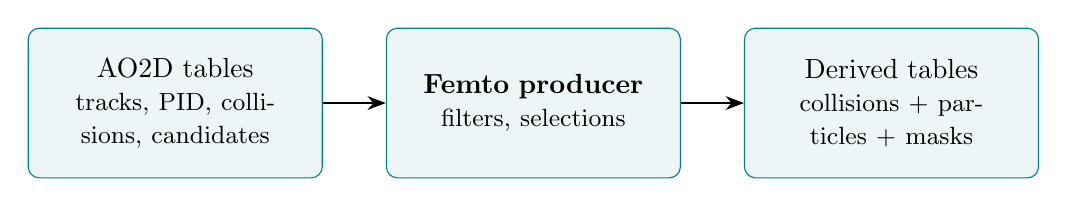
\begin{tikzpicture}[node
                        distance=8mm,box/.style={draw=teal,rounded
                                corners,fill=pale,text width=3.5cm,minimum
                height=19mm,align=center},>=Stealth]
                \node[box] (a) {AO2D tables\\\small tracks, PID,
                collisions, candidates};
                \node[box,right=of a] (b) {\textbf{Femto
                producer}\\\small filters, selections};
                \node[box,right=of b] (c) {Derived tables\\\small
                collisions + particles + masks};
                \draw[->,thick] (a)--(b); \draw[->,thick] (b)--(c);
        \end{tikzpicture}
        \medskip
        \begin{itemize}
                \item Fixed filters and producer acceptance decide
                        which candidates survive.
                \item Configured thresholds become pass/fail
                        decisions in selection masks.
                \item Consumers choose particle samples and build
                        pairs from the derived tables.
        \end{itemize}
        \begin{block}{Bits store comparisons, not detector-observable values}
                Encoding a selection in a bit loses the exact value
                of the detector observable. We only know whether it
                passed the comparison with the configured threshold.
        \end{block}
        \note{The producer delegates to particle builders. Tables
                beyond the compact baseline can be enabled for QA, purity,
                fractions, MC and other uses. Avoid promising a universal
        compression factor.}
        \src{O2Physics/PWGCF/Femto/TableProducer/femtoProducer.cxx}
\end{frame}

\begin{frame}{Which types of selection can we configure?}
        \small A selection compares an observable $x$ with a
        configured value, function or range.
        \medskip
        \footnotesize
        \renewcommand{\arraystretch}{1.25}
        \begin{tabular}{p{.25\textwidth}p{.30\textwidth}p{.35\textwidth}}
                \toprule
                Type & Comparison & Example\\
                \midrule
                Upper / lower limit & $x\leq t$ / $x\geq t$ & TPC
                clusters $\geq90$.\\
                Absolute upper / lower & $|x|\leq t$ / $|x|\geq t$ &
                $|\eta|\leq0.8$.\\
                Function upper / lower & $x\leq f(p_{\mathrm T})$ /
                $x\geq f(p_{\mathrm T})$ & No example so far\\
                Absolute function limit & $|x|\leq f(p_{\mathrm T})$
                / $|x|\geq f(p_{\mathrm T})$ &
                $|\mathrm{DCA}_{xy}|\leq f(p_{\mathrm T})$.\\
                Inside range & $a\leq x\leq b$ & PID range
                $-2<n\sigma_{TPC,proton}<3$.\\
                Outside range & $x<a$ or $x>b$ & Exclude a competing
                mass window.\\
                Equal & $x=t$ & An event-selection flag equals 1.\\
                Equal array & $x_i=t_i$, one bit per element &
                Comparing multiple event flags for trigger selections.\\
                \bottomrule
        \end{tabular}
        \medskip
        \small The comparison type defines \emph{how} a decision is
        evaluated; minimal, optional and neutral define its role in acceptance.
        \note{Based on limits::LimitType in selectionContainer.h.
                Source names are kUpperLimit, kLowerLimit, kAbsUpperLimit,
                kAbsLowerLimit, kUpperFunctionLimit, kLowerFunctionLimit,
                kAbsUpperFunctionLimit, kAbsLowerFunctionLimit, kInsideRange,
                kOutsideRange, kEqual and kEqualArray. Scalar and function
                limits use inclusive comparisons. Equal and EqualArray use an
                epsilon tolerance rather than literal floating-point
                equality. EqualArray compares corresponding entries and
                produces a separate bit for each entry, not one
                all-elements-match bit; trigger selections use this type.
                Ranges use lower;upper strings and can omit a bound. The
                supported comparison type is chosen in the builder
                implementation; users configure the threshold values through
        that builder's options.}
        \src{O2Physics/PWGCF/Femto/Core/selectionContainer.h}
\end{frame}

\begin{frame}{Minimal, optional and neutral: producer semantics}
        \small
        \renewcommand{\arraystretch}{1.35}
        \begin{tabular}{p{.16\textwidth}p{.38\textwidth}p{.37\textwidth}}
                \toprule
                Kind & Effect on producer acceptance & Typical purpose \\
                \midrule
                \textbf{Minimal} & Every configured minimal selection
                must pass its loosest threshold. & Mandatory baseline
                quality; tighter thresholds for later variations.\\
                \textbf{Optional} & Any optional selection passes;
                true if none are configured. & Retain a union of
                candidate hypotheses, e.g. proton \emph{or} pion PID.\\
                \textbf{Neutral} & Neither minimal nor optional: does
                not decide acceptance. & Record decisions for later
                requirements or rejection masks.\\
                \bottomrule
        \end{tabular}
        \begin{block}{Within a selection object, in normal mode}
                \centering
                keep = (all minimal pass) AND (any optional passes)\par
                \small The optional condition is true if no optional
                selections are configured.
        \end{block}
        \note{This formula is scoped to BaseSelection, in addition to
                separate fixed filters. A selection cannot be both minimal
                and optional. The passThrough setting bypasses the normal
                acceptance gate; do not confuse this with relaxing every
                producer filter. Empty groups contribute no condition.
        Neutral bits can be useful in pass-through production.}
        \src{O2Physics/PWGCF/Femto/Core/baseSelection.h;
        O2Physics/PWGCF/Femto/Core/selectionContainer.h}
\end{frame}

\begin{frame}{One selection, three thresholds}
        \centering
        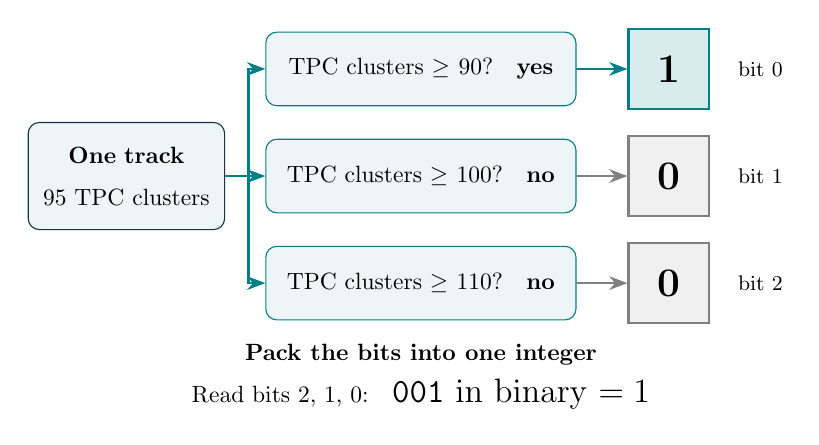
\begin{tikzpicture}[
                        >=Stealth, scale=0.85, transform shape,
                        input/.style={draw=navy,rounded
                                corners,fill=pale,align=center,
                        text width=2.7cm,minimum height=16mm},
                        decision/.style={draw=teal,rounded
                                corners,fill=pale,align=center,
                        text width=4.4cm,minimum height=11mm},
                        bit/.style={draw=teal,thick,minimum
                                width=12mm,minimum height=12mm,
                        font=\LARGE\bfseries,fill=teal!15},
                        flow/.style={->,thick,draw=teal}
                ]
                \node[input] (track) at (0,0) {\textbf{One
                track}\\[2mm]95 TPC clusters};
                \node[decision] (loose) at (4.4,1.6) {TPC clusters
                $\geq 90$?\quad\textbf{yes}};
                \node[decision] (tight) at (4.4,0) {TPC clusters
                $\geq 100$?\quad\textbf{no}};
                \node[decision] (pid) at (4.4,-1.6) {TPC clusters
                $\geq 110$?\quad\textbf{no}};
                \draw[flow] (track.east) -- ++(.35,0) |- (loose.west);
                \draw[flow] (track.east) -- (tight.west);
                \draw[flow] (track.east) -- ++(.35,0) |- (pid.west);
                \node[bit] (b0) at (8.1,1.6) {1};
                \node[bit,fill=gray!12,draw=gray] (b1) at (8.1,0) {0};
                \node[bit,fill=gray!12,draw=gray] (b2) at (8.1,-1.6) {0};
                \node[right=3mm of b0,font=\small] {bit 0};
                \node[right=3mm of b1,font=\small] {bit 1};
                \node[right=3mm of b2,font=\small] {bit 2};
                \draw[flow] (loose.east) -- (b0.west);
                \draw[flow,draw=gray] (tight.east) -- (b1.west);
                \draw[flow,draw=gray] (pid.east) -- (b2.west);
                \node[align=center] at (4.4,-3.0) {\textbf{Pack the
                        bits into one integer}\\[2mm]
                Read bits 2, 1, 0:\quad\Large\texttt{001} in binary $=1$};
        \end{tikzpicture}
        \medskip

        \textbf{1 = passed\qquad 0 = failed}\par
        \small One observable, several thresholds: one bit for each comparison.
        \note{A single observable, the TPC cluster count, is compared
                with three thresholds: 90, 100 and 110. A track with 95
                clusters passes only the first, producing bits 0, 1, 2 equal
                to 1, 0, 0. Read from high bit to low bit: 001, decimal 1.
                This illustrates the encoding before combining different
                observables. Actual minimal selections may omit the
        guaranteed loosest bit; CutCulator supplies the stored mapping.}
        \src{O2Physics/PWGCF/Femto/Core/selectionContainer.h}
\end{frame}

\begin{frame}{Combine different selections in one bitmask}
        \centering
        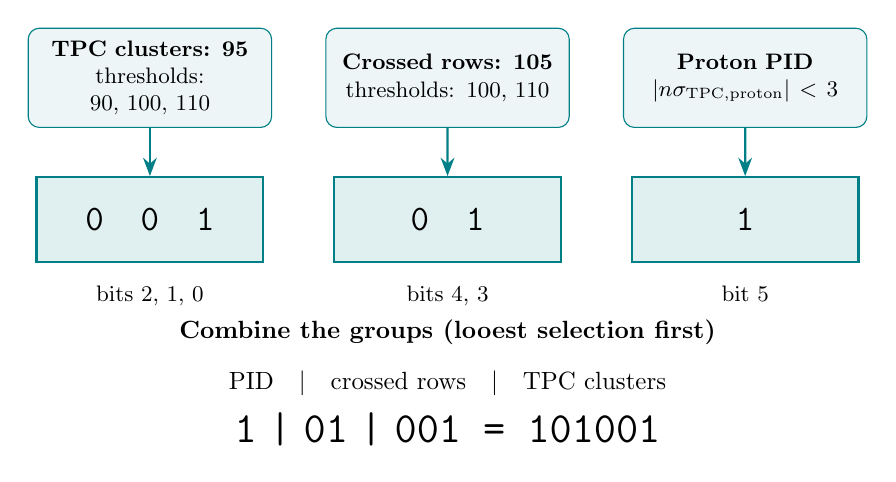
\begin{tikzpicture}[>=Stealth,scale=0.9,transform shape,
                        obs/.style={draw=teal,rounded
                                corners,fill=pale,text width=3.2cm,
                        minimum height=14mm,align=center,font=\small},
                        bits/.style={draw=teal,thick,fill=teal!12,minimum
                                height=12mm,
                minimum width=3.2cm,align=center,font=\Large\ttfamily}]
                \node[obs] (clusters) at (0,1.8) {\textbf{TPC
                clusters: 95}\\thresholds: 90, 100, 110};
                \node[obs] (rows) at (4.2,1.8) {\textbf{Crossed rows:
                105}\\thresholds: 100, 110};
                \node[obs] (pid) at (8.4,1.8) {\textbf{Proton
                PID}\\$|n\sigma_{\mathrm{TPC,proton}}|<3$};
                \node[bits] (c) at (0,-.2) {0\quad0\quad1};
                \node[bits] (r) at (4.2,-.2) {0\quad1};
                \node[bits] (p) at (8.4,-.2) {1};
                \draw[->,thick,teal] (clusters)--(c);
                \draw[->,thick,teal] (rows)--(r);
                \draw[->,thick,teal] (pid)--(p);
                \node[below=2mm of c,font=\small] {bits 2, 1, 0};
                \node[below=2mm of r,font=\small] {bits 4, 3};
                \node[below=2mm of p,font=\small] {bit 5};
                \node[align=center] at (4.2,-2.5) {\textbf{Combine
                        the groups (looest selection first)}\\[3mm]
                        PID\quad$|$\quad crossed rows\quad$|$\quad
                        TPC clusters\\[2mm]
                \LARGE\texttt{1\;|\;01\;|\;001 = 101001}};
        \end{tikzpicture}
        \medskip

        All decisions are stored together as one integer: binary
        \texttt{101001} $=41$.
        \par\small Illustrative mapping; actual positions come from
        the producer configuration.
        \note{Continue the 95-TPC-cluster example from the previous
                slide. Crossed rows are a second observable with thresholds
                100 and 110, giving local bits 01 for a track with 105 rows.
                These occupy global positions 3 and 4. The proton PID
                decision occupies bit 5. Combining the disjoint groups with
                bitwise OR gives 101001 in binary, decimal 41. The separators
                only visualize the groups; they are not part of the stored
        integer. Actual production may omit guaranteed minimal bits.}
        \src{O2Physics/PWGCF/Femto/Core/baseSelection.h;
        O2Physics/PWGCF/Femto/Core/selectionContainer.h}
\end{frame}



\begin{frame}[shrink=8]{What survives? Quality cuts and PID together}
        \small
        A stored particle has passed every loosest minimal selection,
        so these guaranteed decisions need no bits; particles failing
        even one minimal selection are not stored.
        A particle failing all optional selections are also not stored.
        \medskip\par
        \textbf{Three minimal quality selections} (baseline / tighter
        threshold):
        \par TPC clusters: $\geq 90$ / $\geq 100$;\quad crossed rows:
        $\geq 100$ / $\geq 110$;\quad ITS clusters: $\geq 5$ / $\geq 6$.
        \medskip\par
        Optional selections: proton PID or pion PID.
        \medskip
        \centering
        \renewcommand{\arraystretch}{1.3}
        \begin{tabular}{cccccc l}
                \toprule
                Track & TPC clusters & Crossed rows & ITS clusters &
                Proton PID & Pion PID & Producer\\
                \midrule
                1 & 95 & 105 & 5 & pass & fail & keep\\
                2 & 110 & 115 & 6 & fail & pass & keep\\
                \textbf{3} & \textbf{80} & 115 & 6 & pass & fail &
                \textbf{discard}\\
                4 & 110 & 115 & 6 & \textbf{fail} & \textbf{fail} &
                \textbf{discard}\\
                \bottomrule
        \end{tabular}
        \medskip
        \begin{block}{Why are tracks 3 and 4 discarded?}
                Track 3 passes proton PID but fails the minimal
                selection of 90 TPC clusters.\par
                Track 4 passes all minimal selections but no optional
                PID selection.
        \end{block}
        \note{Illustrative configuration, not the installed defaults.
                The three quality observables are minimal; each has a loose
                baseline and a tighter working point. Track 1 passes all
                loose thresholds and proton PID but fails every tighter
                quality threshold. Track 2 passes all tighter quality
                thresholds and pion PID. Track 3 passes proton PID,
                crossed-row and ITS-cluster requirements, but has only 80 TPC
                clusters and fails the minimal requirement of at least 90.
                Track 4 passes quality but neither optional PID hypothesis,
                so it is discarded. The guaranteed loosest minimal decisions
                may have no stored bit; tighter decisions are available to
        consumers through masks.}
        \src{O2Physics/PWGCF/Femto/Core/baseSelection.h;
                O2Physics/PWGCF/Femto/Core/selectionContainer.h;
        O2Physics/PWGCF/Femto/Core/trackBuilder.h}
\end{frame}

\begin{frame}[fragile,shrink=8]{CutCulator: where to find it and what to open}
        CutCulator is a convenient tool to compute the selection
        bitmasks needed for our analysis.
        \medskip\par
        Start with the graphical interface in the O2Physics source:
 \begin{lstlisting}[language=bash]
 # Graphical interface (GUI)
 python3 $HOME/alice/O2Physics/PWGCF/Femto/Macros/cutculator_gui.py
 \end{lstlisting}
        \begin{enumerate}
                \item Obtain \texttt{AnalysisResults.root} from the producer.
                \item Choose the relevant collision or particle
                        \textbf{selection histogram}.
                \item Select thresholds and read the resulting mask.
        \end{enumerate}
        \begin{block}{The producer stores its full configuration in the file}
                The producer writes its full selection configuration,
                including selection thresholds, bit positions and filters,
                into \texttt{AnalysisResults.root}. All this information
                can be visualized with CutCulator; the producer JSON is
                not needed to compute the selection masks.
        \end{block}
        \small Filter histograms show already-applied settings; they
        have no selectable bits.
        \note{Use the O2Physics source checkout, not an assumed
                executable on PATH. PyROOT is required; the GUI also needs
                tkinter and a graphical display. Hyperloop output must
                include the producer metadata: consumer-only histograms or
        the derived AO2D alone are insufficient for these tools.}
        \src{O2Physics/PWGCF/Femto/Macros/cutculator_gui.py}
\end{frame}

\begin{frame}[fragile,shrink=8]{CutCulator with the GUI}
        \small
 \begin{lstlisting}[language=bash]
 python3 "$HOME/alice/O2Physics/PWGCF/Femto/Macros/cutculator_gui.py" \
   AnalysisResults.root --dir femto-producer
 \end{lstlisting}
\begin{enumerate}\setlength{\itemsep}{1pt}
                \item Open the producer ROOT file and choose the
                        selection histogram.
                \item Inspect the minimal, optional and neutral
                        groups; check the desired cuts.
                \item Copy the computed mask into the consumer configuration.
                \item For systematic scans, use the variation export
                        to save JSON.
        \end{enumerate}
        \begin{block}{A working point versus a scan}
                The combined mask requires all checked bits.
                Variation export lists alternative working points as JSON.
        \end{block}
        \vspace{-2mm}
        \footnotesize The GUI needs PyROOT, \texttt{tkinter}, and a
        desktop/display.\par
        \textbf{Linux:} \texttt{tkinter} may already be installed;
        otherwise use the distribution's Python/Tk package.\par
        \textbf{macOS:} Homebrew provides \texttt{python-tk@X.Y};
        match the Python version used in the O2Physics environment.
        \note{The local GUI contains systematic-variation export.
                Demonstrate one working point first, then two alternatives on
                one axis. Exporting variations does not launch O2 tasks. A
                neutral selection is not automatically a veto: copy its mask
                into a rejectionMask field to use it as one. Test tkinter
                with python3 -m tkinter in the same environment that provides
                PyROOT. tkinter is an optional Python standard-library module
                with a compiled extension, not a pip-installable dependency.
                On macOS a Homebrew Tk package must match the Homebrew Python
                in use; installing it does not add Tk support to an unrelated
                O2Physics Python build. References:
                https://docs.python.org/3/library/tkinter.html and
        https://formulae.brew.sh/formula/python-tk@3.14.}
        \src{O2Physics/PWGCF/Femto/Macros/cutculator_gui.py}
\end{frame}

\begin{frame}[shrink=8]{CutCulator GUI: open a ROOT file}
        \centering
        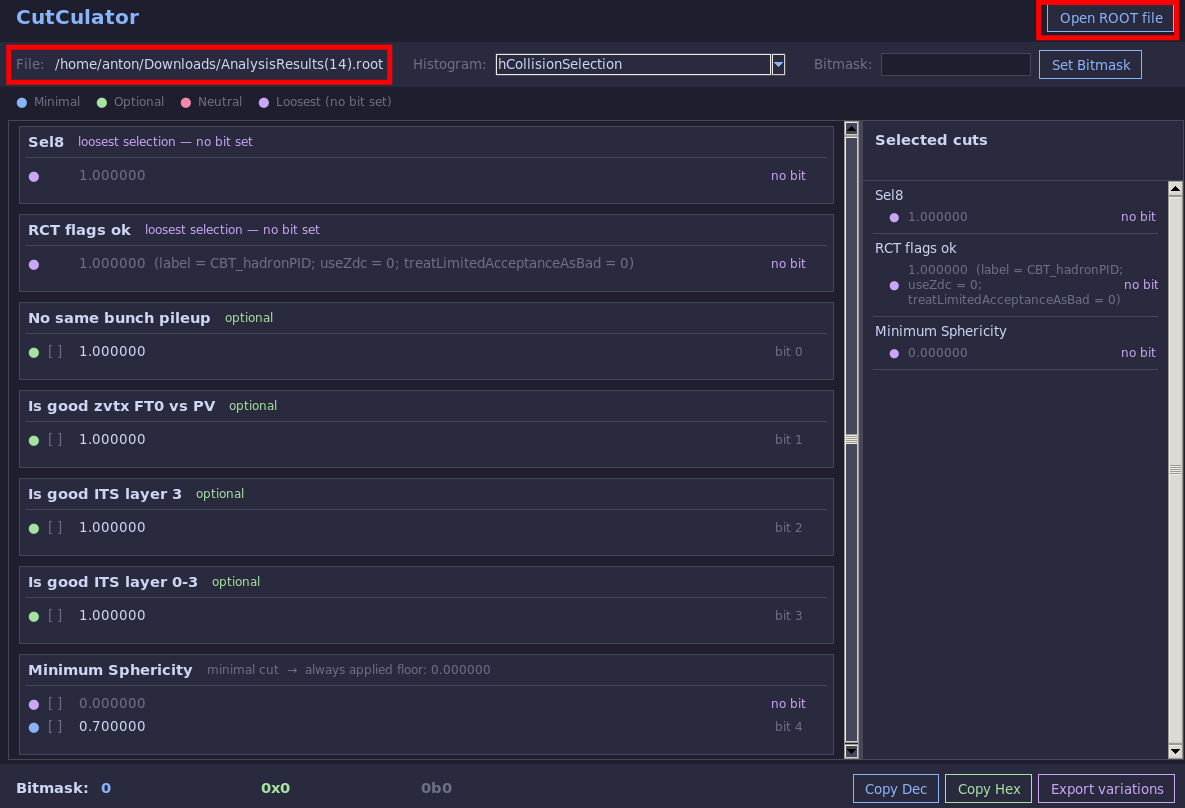
\includegraphics[width=\textwidth,height=0.82\textheight,keepaspectratio]{slides/assets/cutculator-gui-open.png}
        \medskip

        \small Click \textbf{Open ROOT file} to choose a file
        interactively; its path appears next to \textbf{File:}.
        \note{Screenshot supplied by the presenter. The red
                highlights identify the Open ROOT file button at the top
                right and the active file path at the top left. The GUI can
                be launched without a file argument and the producer output
        selected interactively.}
\end{frame}

\begin{frame}[shrink=8]{CutCulator GUI: choose the selection histogram}
        \centering
        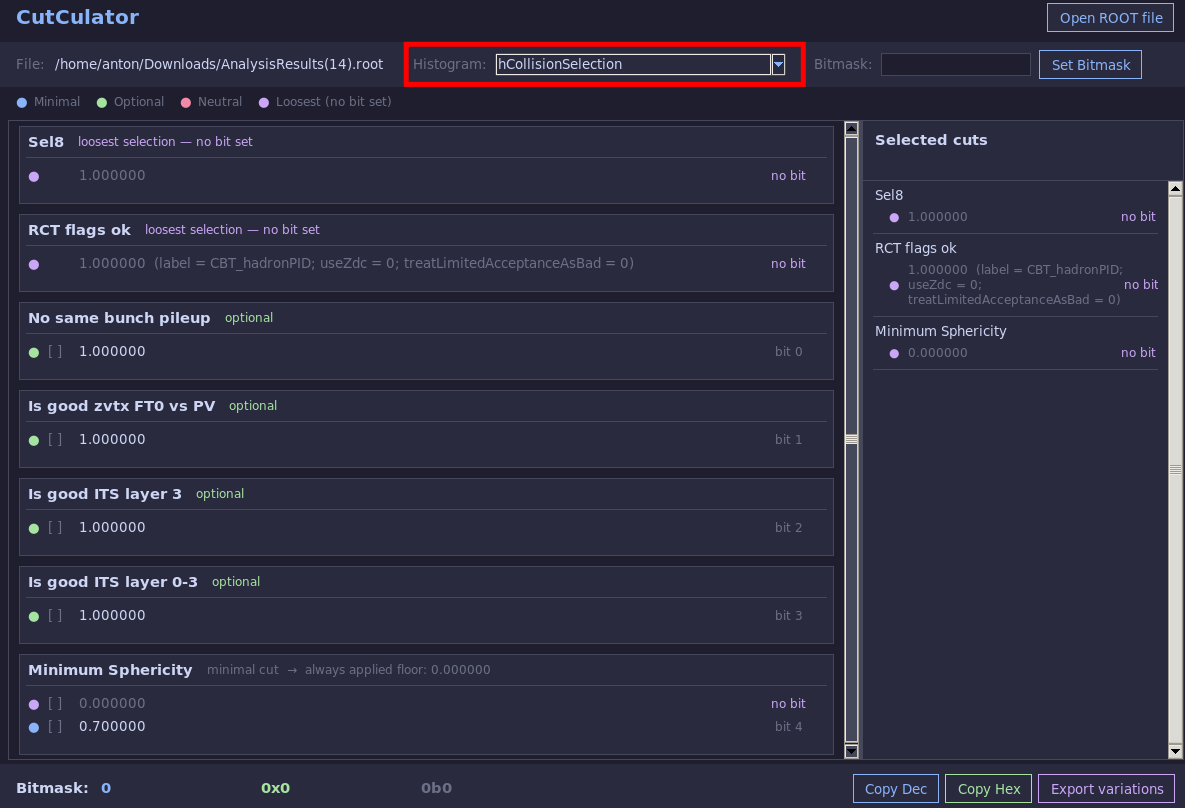
\includegraphics[width=\textwidth,height=0.82\textheight,keepaspectratio]{slides/assets/cutculator-gui-histogram.png}
        \medskip

        \small Use the \textbf{Histogram} dropdown to choose
        collision, track or candidate selections.
        \note{Screenshot supplied by the presenter. The red highlight
                identifies the histogram dropdown, currently showing
                hCollisionSelection. Choose hTrackSelection for tracks,
                hLambdaSelection for Lambda candidates, or the other
        selection histogram corresponding to the desired particle sample.}
\end{frame}

\begin{frame}{CutCulator GUI: select cuts and copy the mask}
        \centering
        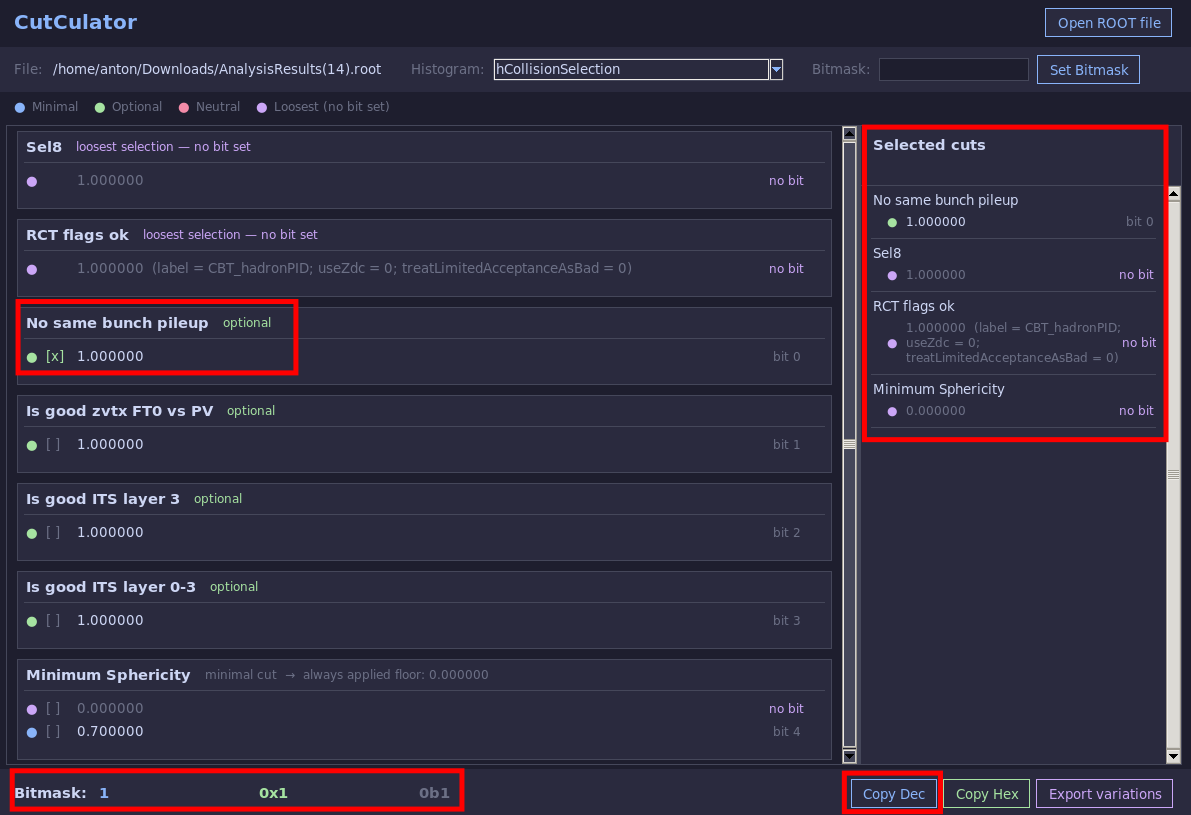
\includegraphics[width=\textwidth,height=0.75\textheight,keepaspectratio]{slides/assets/cutculator-gui-selection.png}
        \medskip

        \small Check a selection on the \textbf{left}; review its
        summary under \textbf{Selected cuts} on the right.\par
        The \textbf{Bitmask} updates at the bottom; use \textbf{Copy
        Dec} or \textbf{Copy Hex} to copy it.
        \note{Screenshot supplied by the presenter. The highlighted
                No same bunch pileup option is selected, setting bit 0. The
                Selected cuts panel lists the chosen decision along with the
                always-applied no-bit floors. The bottom status shows the
                updated mask as decimal 1, hexadecimal 0x1 and binary 0b1.
        Copy Dec copies the decimal form; Copy Hex copies the hexadecimal form.}
\end{frame}

\begin{frame}{CutCulator GUI: inspect a filter histogram}
        \centering
        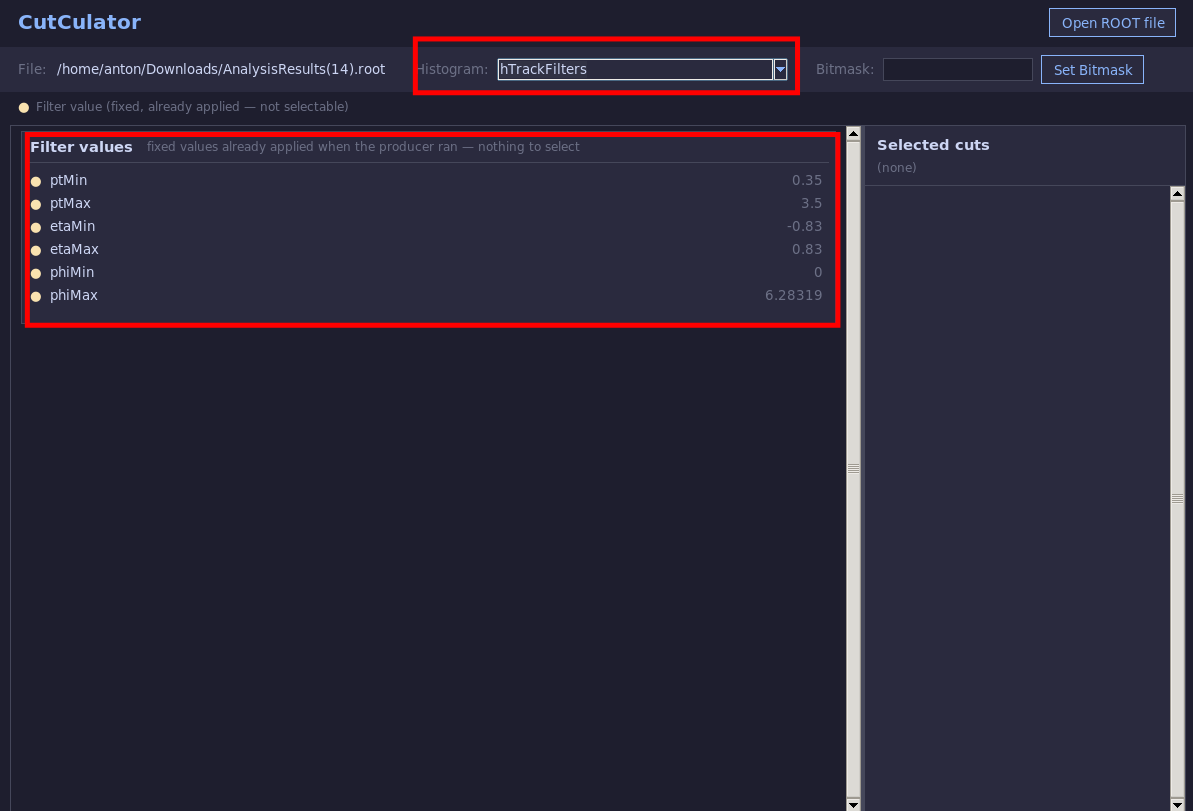
\includegraphics[trim=0 460 0
        0,clip,width=\textwidth,height=0.65\textheight,keepaspectratio]{slides/assets/cutculator-gui-filters.png}
        \medskip

        \raggedright
        Choose \texttt{hTrackFilters} to inspect the producer's track
        prefilters.
        \begin{itemize}
                \item The displayed values were already applied
                        during production.
                \item They are read-only: there are no selection bits
                        to choose here.
        \end{itemize}
        \note{Screenshot supplied by the presenter. The image is
                clipped in LaTeX to omit the empty lower part of the window.
                The highlighted dropdown shows hTrackFilters; the values
                panel records ptMin, ptMax, etaMin, etaMax, phiMin and phiMax
                from this production. Unlike a selection histogram, this view
        offers no checkboxes and no bitmask choices.}
        \src{O2Physics/PWGCF/Femto/Macros/cutculator_gui.py}
\end{frame}

\begin{frame}[fragile,shrink=8]{Optional: a terminal-only CutCulator}
        A terminal-only version is available when needed, for example
        over SSH without a graphical display. It computes the same selection
        masks; the GUI is generally easier to use.
        \medskip\par
 \begin{lstlisting}[language=bash]
 O2PHYSICS_SRC="$HOME/alice/O2Physics"
 python3 "$O2PHYSICS_SRC/PWGCF/Femto/Macros/cutculator.py" \
   AnalysisResults.root
 \end{lstlisting}

 \begin{lstlisting}[language=bash]
 # Inspect the cuts represented by an existing mask:
 python3 "$O2PHYSICS_SRC/PWGCF/Femto/Macros/cutculator.py" \
   AnalysisResults.root --bitmask
 \end{lstlisting}
        \small Decode mode asks for the histogram and then the mask.\par
        \note{TUI here means line-based terminal prompts. Indices are
                generated from the file, so demonstrate rather than hard-code
                an index. A no-bit minimal floor contributes zero to the mask
                but is still in effect. The --bitmask flag is verified in
        this local checkout and may differ in other versions.}
        \src{O2Physics/PWGCF/Femto/Macros/cutculator.py}
\end{frame}

\begin{frame}{CutCulator in the terminal: choosing a histogram}
        \centering
        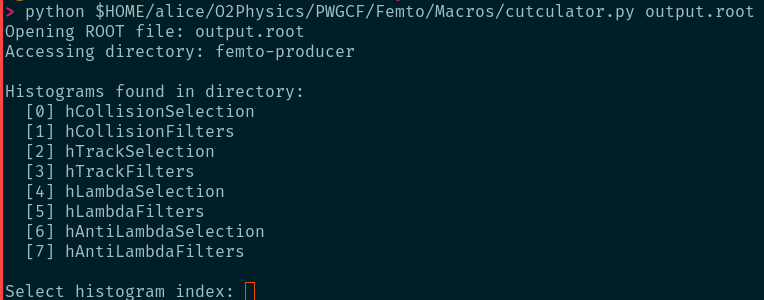
\includegraphics[width=\textwidth,height=0.66\textheight,keepaspectratio]{slides/assets/cutculator-terminal.png}
        \medskip

        \raggedright
        \textbf{Example:} enter \texttt{2} for
        \texttt{hTrackSelection}, or \texttt{4} for
        \texttt{hLambdaSelection}.\par
        \small The indices depend on the histograms in your producer output.
        \note{Screenshot supplied by the presenter. Here the producer
                QA file is called output.root. It contains the same kind of
                selection metadata described for AnalysisResults.root. Choose
                a selection histogram to compute a mask; filter histograms
        only describe fixed prefilters.}
\end{frame}

\begin{frame}{CutCulator in the terminal: selected cuts and final mask}
        \begin{columns}[c]
                \begin{column}{.67\textwidth}
                        \centering
                        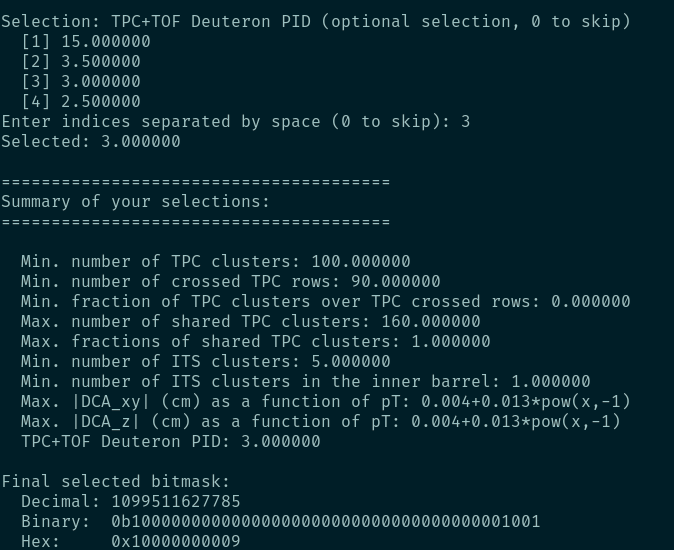
\includegraphics[width=\textwidth,height=0.85\textheight,keepaspectratio]{slides/assets/cutculator-summary.png}
                \end{column}
                \begin{column}{.30\textwidth}
                        \small
                        \textbf{Check the selected cuts}\par
                        The summary lists the thresholds chosen for the sample.
                        \medskip

                        \textbf{Read the final mask}\par
                        Decimal, binary and hexadecimal are three
                        representations of the same integer.
                        \medskip

                        Copy the mask into the corresponding
                        particle-selection configurable.
                \end{column}
        \end{columns}
        \note{Screenshot supplied by the presenter. This example
                selects a TPC+TOF deuteron PID threshold of 3 and prints the
                chosen track-quality and PID selections followed by the final
                mask. The mask is specific to this producer's configuration
                and must not be reused for a different production without
        checking its metadata.}
\end{frame}

\section{Example 1: proton--$\Lambda$ from AO2D}

\begin{frame}{Example 1: proton--$\Lambda$ from AO2D}
 \begin{block}{Our goal}
 Produce a proton--$\Lambda$ correlation function, starting from an AO2D.
 \end{block}
 \begin{enumerate}
 \item \textbf{Part 1:} producer configuration for collisions, protons and $\Lambda$.
 \item \textbf{Part 2:} proton and $\Lambda$ QA.
 \item \textbf{Part 3:} proton--$\Lambda$ pairing and correlation.
 \end{enumerate}
 \medskip
 \textbf{Complete example files:} \texttt{examples/01-proton-lambda/}\par
 \small The final run script and configuration already contain every task; their settings evolve step by step during the live demonstration.
 \note{Instructor-led demonstrations, not exercises. This example implements the complete proton-Lambda chain, introduced through five live steps. The supplied input is a Run 3 pp data AO2D, LHC26ad, run 570703.}
 \src{O2Physics/PWGCF/Femto/TableProducer/femtoProducer.cxx; O2Physics/PWGCF/Femto/Tasks/femtoTrackQa.cxx}
\end{frame}


\begin{frame}[fragile]{Part 1: collision filters}
 \begin{lstlisting}
 "CollisionFilter": {
   "vtxZMin": "-10", "vtxZMax": "10",
   "multMin": "0",   "multMax": "5000",
   "centMin": "0",   "centMax": "100",
   "magFieldMin": "-5", "magFieldMax": "5"
 }
 \end{lstlisting}
 \begin{itemize}
 \item In this example the vertex range is $-10\leq z_{\rm vtx}\leq10$ cm; multiplicity and centrality bounds are broad.
 \item Magnetic-field bounds are in kG. Further options include sphericity and the MC sub-generator ID.
 \end{itemize}
 \note{The prefix is CollisionFilter, singular, unlike TrackFilters. This is an excerpt from the actual example configuration. The collision builder uses inclusive bounds. subGeneratorId=-1 disables that MC-specific filter. In normal production a failed collision filter prevents the event from entering the produced collision sample.}
 \src{O2Physics/PWGCF/Femto/Core/collisionBuilder.h}
\end{frame}

\begin{frame}[fragile]{Part 1: collision selection flags}
 \begin{lstlisting}
 "CollisionBits": {
   "passThrough": "false",
   "sel8": "-1",
   "rctFlags": "1",
   "noSameBunchPileup": "0"
 }
 \end{lstlisting}
 \small Integer settings control the role of these event-selection flags:
 \par\medskip
 \renewcommand{\arraystretch}{1.2}
 \begin{tabular}{cll}
 \toprule
 Value & Role & Producer behavior\\
 \midrule
 \texttt{"1"} & Minimal & Required; its guaranteed bit is omitted.\\
 \texttt{"-1"} & Optional & Stored as a bit; contributes to the optional OR.\\
 \texttt{"0"} & Disabled & Neither applied nor stored.\\
 \bottomrule
 \end{tabular}
 \par\medskip
 \small RCT is minimal; \texttt{sel8} is optional; \texttt{noSameBunchPileup} is disabled. The RCT quality definition is configured separately.
 \note{These are the boolean collision-flag settings, not the table-output auto/off/on switches. The optional OR follows the same BaseSelection rule described earlier. CollisionBits also supports vectors of occupancy/sphericity thresholds and trigger selections. hCollisionSelection records the metadata. CollisionBits.passThrough is separate from TrackBits.passThrough.}
 \src{O2Physics/PWGCF/Femto/Core/collisionBuilder.h; O2Physics/PWGCF/Femto/Core/baseSelection.h}
\end{frame}

\begin{frame}[fragile]{Part 1: RCT quality requirements}
 \begin{lstlisting}
 "CollisionBits": {"rctFlags": "1"},
 "CollisionRctFlags": {
   "label": "CBT_hadronPID",
   "useZdc": "false",
   "treatLimitedAcceptanceAsBad": "false"
 }
 \end{lstlisting}
 \small \texttt{CBT\_hadronPID} is our usual choice: it checks FT0, ITS, TPC tracking/PID and TOF quality.
 \begin{itemize}
 \item Other presets include \texttt{CBT}, \texttt{CBT\_electronPID}, \texttt{CBT\_calo}, \texttt{CBT\_muon} and \texttt{CBT\_muon\_glo}.
 \item \texttt{useZdc} additionally includes ZDC quality, relevant for Pb--Pb.
 \item We usually keep limited-acceptance periods when the limitation is reproducible in MC: \texttt{treatLimitedAcceptanceAsBad = "false"}.
 \end{itemize}
 \note{CollisionBits.rctFlags controls the selection role; CollisionRctFlags controls which RCT requirements are checked. The preset label selects a detector-quality combination, not a particle PID cut. In the example rctFlags=1 makes it minimal. The local RCTFlagsChecker defines the available preset labels.}
 \src{O2Physics/PWGCF/Femto/Core/collisionBuilder.h; O2Physics/Common/CCDB/RCTSelectionFlags.h}
\end{frame}

\begin{frame}[fragile]{Part 1: configurable trigger selections}
 \begin{lstlisting}
 "CollisionBits": {
   "triggers": {"values": ["triggerName1", "triggerName2"]},
   "triggerBcTolerance": "100"
 },
 "ConfCcdb": {"triggerPath": "EventFiltering/Zorro/"}
 \end{lstlisting}
 \small The names above are illustrative; the available trigger names depend on the production.
 \begin{itemize}
 \item Zorro provides one decision for each configured trigger, matched in bunch crossings within the configured tolerance.
 \item Trigger decisions are encoded as \textbf{equal-array} selections: one bit per trigger, each compared with \texttt{"1"}.
 \item Trigger decisions are \textbf{optional}: when they are the only optional selections, only events firing at least one configured trigger are stored.
 \end{itemize}
 \small The current example has an empty trigger list.
 \note{This is an illustrative trigger configuration, not a change to the supplied minimum-bias example. CollisionBits.triggers defaults to an empty vector. ConfCcdb.triggerPath selects the Zorro CCDB location, and triggerBcTolerance controls matching around the collision global BC. CutCulator shows the trigger names in the selection metadata. A consumer can explicitly require particular stored trigger bits; configuring optional triggers alongside sel8 does not require both.}
 \src{O2Physics/PWGCF/Femto/Core/collisionBuilder.h; O2Physics/PWGCF/Femto/Core/selectionContainer.h}
\end{frame}

\begin{frame}[fragile]{Part 1: minimal track-quality selections}
 \small In \texttt{examples/01-proton-lambda/configuration.json}, under \texttt{femto-producer}:
 \begin{lstlisting}
 "TrackFilters": {
   "ptMin": "0.3", "ptMax": "4.0",
   "etaMin": "-0.8", "etaMax": "0.8"
 },
 "TrackBits": {
   "tpcClustersMin":    {"values": ["90", "100", "110"]},
   "tpcCrossedRowsMin": {"values": ["80", "100", "110"]},
   "itsClustersMin":    {"values": ["5", "6"]},
   "itsIbClustersMin":  {"values": ["1"]}
 }
 \end{lstlisting}
 \begin{itemize}
 \item These quality observables are \textbf{minimal} selections in the builder.
 \item Every retained standalone track passes each loosest threshold.
 \item Tighter thresholds are recorded as bits for later working points.
 \end{itemize}
 \small The full configuration also includes DCA selections and shared-cluster limits.
 \note{The JSON on this slide is an excerpt, not a replacement for the complete configuration. The minimal/optional/neutral role is defined by addSelection in TrackSelection::configure. Changing the vector values does not change that role. TrackBits.passThrough remains false.}
 \src{O2Physics/PWGCF/Femto/Core/trackBuilder.h}
\end{frame}

\begin{frame}[fragile]{Part 1: proton PID optional, pion PID neutral}
 \begin{lstlisting}
 "requirePidProton": "true",
 "tpcProton":    {"values": ["-3;3", "-2.5;2.5"]},
 "tpctofProton": {"values": ["3.0", "2.5"]},
 "requirePidPion": "false",
 "tpcPion":      {"values": ["-3;3"]}
 \end{lstlisting}
 \begin{itemize}
 \item \texttt{requirePidProton = "true"}: configured proton PID decisions become \textbf{optional} selections for producer acceptance.
 \item \texttt{requirePidPion = "false"}: configured pion PID decisions remain \textbf{neutral}; pion PID cannot admit a track by itself.
 \item Retained proton candidates still carry the pion PID decision, so we can apply a pion veto later with a rejection mask.
 \end{itemize}
 \small The same \texttt{requirePid*} pattern exists for the other species.
 \note{Only proton requirePid is true in this example. The optional conditions are ORed in the producer, while minimal quality must all pass. Neutral does not mean the bit is a veto automatically: the consumer must explicitly put it in a rejectionMask. The local builder evaluates PID a second time for accepted tracks to populate competing-hypothesis bits. No pion rejection is applied in the initial QA run.}
 \src{O2Physics/PWGCF/Femto/Core/trackBuilder.h}
\end{frame}

\begin{frame}[fragile]{Part 1: set the TOF threshold already in the producer}
 \begin{lstlisting}
 # Producer: TrackBits
 "minMomTofProton": "0.75"
 # Consumer: TrackSelection1
 "pidThres": "0.75"
 \end{lstlisting}
 \begin{itemize}
 \item Below $p=0.75$ GeV/$c$: proton PID can use TPC information.
 \item At and above the producer threshold: a track without TOF cannot pass the proton optional selections.
 \item Rejecting these tracks before storing them reduces the derived-data size.
 \end{itemize}
 \begin{block}{The consumer can choose a lower threshold}
 All configured PID decisions are evaluated for retained candidates, so the consumer's \texttt{pidThres} can also be lower than the producer's \texttt{minMomTofProton}.
 \end{block}
 \note{These are total-momentum thresholds, not transverse momentum. In the local implementation the producer gate uses p >= threshold, while the consumer uses the low mask at p <= pidThres. TOF presence alone does not impose a combined PID cut: the example QA consumer explicitly requires the TPCTOF bit at high momentum. With only requirePidProton enabled, another species cannot rescue a high-p track without TOF. If additional optional species are enabled, their acceptance can change which tracks survive.}
 \src{O2Physics/PWGCF/Femto/Core/trackBuilder.h; O2Physics/PWGCF/Femto/Core/partitions.h}
\end{frame}

\begin{frame}[fragile]{Part 1: $\Lambda$ filters}
 \begin{lstlisting}
 "V0Filters": {
   "ptMin": "0.3", "ptMax": "6",
   "etaMin": "-0.8", "etaMax": "0.8",
   "massMinLambda": "1.08", "massMaxLambda": "1.16"
 }
 \end{lstlisting}
 \begin{itemize}
 \item V0 candidates are reconstructed from a pair of oppositely charged daughter tracks.
 \item The filters define the candidate kinematic acceptance and a broad $\Lambda$ mass window.
 \item Topology, daughter quality and daughter PID are handled by \texttt{LambdaBits}.
 \end{itemize}
 \note{Candidate filters use the Lambda mass hypothesis. Daughter-index dependencies require the track table even without standalone-track QA. The process-function choices are explained on their own slide after the selection configuration.}
 \src{O2Physics/PWGCF/Femto/TableProducer/femtoProducer.cxx; O2Physics/PWGCF/Femto/Core/v0Builder.h}
\end{frame}

\begin{frame}[fragile]{Part 1: $\Lambda$ selection bits and K$^0_{\rm S}$ rejection}
 \begin{lstlisting}
 "LambdaBits": {
   "cpaMin":          {"values": ["0.99", "0.995"]},
   "dcaDauMax":       {"values": ["1.5", "1.0"]},
   "dauTpcClustersMin": {"values": ["80"]},
   "posDauTpcProton": {"values": ["5", "3"]},
   "negDauTpcPion":   {"values": ["5", "3"]},
   "rejectK0shortMassRanges": {"values": ["0.475;0.515"]}
 }
 \end{lstlisting}
 \small For $\Lambda\to p\pi^-$, the daughters follow the proton and pion hypotheses. The K$^0_{\rm S}$ rejection instead tests their reconstructed $\pi^+\pi^-$ mass: candidates inside $0.475$--$0.515$ GeV/$c^2$ are rejected.
 \begin{block}{No K$^0_{\rm S}$ rejection}
 \texttt{"rejectK0shortMassRanges": \{"values": [";"]\}}\par
 A plain \texttt{";"} means no excluded mass range: every candidate passes this rejection selection.
 \end{block}
 \note{These selections are minimal in normal production. The configured K0short rejection decision passes when the candidate lies outside the excluded mass interval. The current one-entry rejection range is the guaranteed minimal baseline and carries no stored bit; tighter configured alternatives can carry bits. Replacing its only range by ";" disables rejection without changing the four tighter bits used by the example's mask 15. The full JSON also includes daughter eta/DCA, radius and decay-vertex selections.}
 \src{O2Physics/PWGCF/Femto/Core/v0Builder.h; O2Physics/PWGCF/Femto/Core/selectionContainer.h}
\end{frame}

\begin{frame}{Part 1: open-ended acceptance and rejection ranges}
 \small Ranges have the form \texttt{"lower;upper"}. Either limit may be omitted.
 \medskip
 \footnotesize
 \renewcommand{\arraystretch}{1.1}
 \begin{tabular}{p{.14\textwidth}p{.37\textwidth}p{.39\textwidth}}
 \toprule
 Bounds & Acceptance: TPC PID & Rejection: competing mass $m$\\
 \midrule
 Both & \texttt{"-3;3"}\newline accepts $-3\leq n\sigma\leq3$ & \texttt{"0.475;0.515"}\newline rejects $0.475\leq m\leq0.515$\\
 Upper only & \texttt{";3"}\newline accepts $n\sigma\leq3$ & \texttt{";0.515"}\newline rejects $m\leq0.515$\\
 Lower only & \texttt{"-3;"}\newline accepts $n\sigma\geq-3$ & \texttt{"0.475;"}\newline rejects $m\geq0.475$\\
 Neither & \texttt{";"}\newline accepts every value & \texttt{";"}\newline rejects no value\\
 \bottomrule
 \end{tabular}
 \medskip
 \small
 \begin{block}{The meaning depends on the selection type}
 Acceptance tests \textbf{inside} the range; rejection tests \textbf{outside}. With \texttt{";"}, every value passes either selection.
 \end{block}
 \note{Acceptance corresponds to kInsideRange and rejection to kOutsideRange. Nonempty bounds are inclusive for the accepted/excluded interval; the outside decision is strict. Missing lower/upper bounds extend to minus/plus infinity in the conceptual description. The completely open rejection range ";" is a deliberate special case in parseRangeString: it denotes reject nothing, rather than excluding the entire real line. This table describes the individual selection decision, independent of its minimal/optional/neutral role. Mass values are in GeV/c2.}
 \src{O2Physics/PWGCF/Femto/Core/selectionContainer.h}
\end{frame}

\begin{frame}[fragile]{Part 1: TOF PID for $\Lambda$ daughters}
 \begin{lstlisting}
 "LambdaBits": {
   "posDauTofProton": {"values": ["5", "3"]},
   "negDauTofPion":   {"values": ["5", "3"]},
   "requireTof": "true",
   "keepTracksWithoutTof": "true"
 }
 \end{lstlisting}
 \begin{itemize}
 \item \texttt{requireTof}: makes the configured daughter TOF cuts mandatory.
 \item \texttt{keepTracksWithoutTof}: keeps daughters without a TOF signal.
 \end{itemize}
 \begin{block}{With a TOF signal}
 A measured TOF value that fails the mandatory cut still rejects the candidate.
 \end{block}
 \note{Illustrative extension, not enabled in the supplied baseline JSON: adding TOF thresholds can change mask assignments, which must be recomputed with CutCulator. With requireTof false, the TOF decisions are neutral and do not reject candidates at producer level; consumers may still select their bits. For anti-Lambda the positive daughter uses the pion hypothesis and the negative daughter the proton hypothesis. keepTracksWithoutTof overrides missing-signal failure only, not an actually measured PID failure.}
 \src{O2Physics/PWGCF/Femto/Core/v0Builder.h}
\end{frame}

\begin{frame}[fragile]{Part 1: producer process functions}
 \small
 \begin{lstlisting}
 "femto-producer": {
   "processTracksRun3pp": "false",
   "processTracksV0sRun3pp": "true"
 }
 \end{lstlisting}
 \begin{itemize}
 \item The process function defines the \textbf{data subscriptions}. Track-only processing subscribes to track inputs, without V0, cascade, kink or photon candidates.
 \item Processes handling V0s, cascades, kinks or photons require the corresponding input tables and builder/helper tasks in the analysis chain.
 \item The current producer has \textbf{no Run 2 process functions}. Run 3 variants cover pp and Pb--Pb, with data and MC options.
 \end{itemize}
 \begin{block}{Run 3 systems: the centrality estimator}
 pp uses \textbf{FT0M}; Pb--Pb uses \textbf{FT0C}.
 \end{block}
 \note{Track-only means only the track candidate category: the process also needs collision, event-selection, multiplicity and PID inputs. Process signatures determine subscriptions and therefore which upstream builders are needed; output-table switches alone do not activate candidate processing. The main pp/PbPb distinction discussed here is the centrality estimator stored by CollisionSelection::setCentrality: FT0M for kPP_Run3, FT0C for kPbPb_Run3. The local producer currently exposes Run 3 processing functions only. The final supplied configuration enables processTracksV0sRun3pp and disables processTracksRun3pp and the other producer processes.}
 \src{O2Physics/PWGCF/Femto/TableProducer/femtoProducer.cxx; O2Physics/PWGCF/Femto/Core/collisionBuilder.h}
\end{frame}

\begin{frame}[fragile]{Part 2: track QA -- particle and kinematic selections}
 \small Under \texttt{femto-track-qa}:
 \begin{lstlisting}
 "TrackSelection1": {
   "pdgCodeAbs": "2212", "chargeSign": "1", "chargeAbs": "1",
   "ptMin": "0.3", "ptMax": "4.0",
   "etaMin": "-0.8", "etaMax": "0.8",
   "phiMin": "0", "phiMax": "6.28318548"
 }
 \end{lstlisting}
 \begin{itemize}
 \item \texttt{chargeAbs}: rescales stored $p_{\mathrm T}/|Z|$ to physical momentum; \texttt{"2"} for $^3$He, usually \texttt{"1"}.
 \item \texttt{chargeSign}: \texttt{"1"} positive, \texttt{"-1"} negative, \texttt{"0"} both.
 \item \texttt{pdgCodeAbs}: supplies the four-vector mass for every species; PID is selected separately by masks.
 \end{itemize}
 \begin{block}{Antiparticles}
 \footnotesize Antiproton: \texttt{"chargeSign": "-1"}; \texttt{pdgCodeAbs} stays \texttt{"2212"}.
 \end{block}
 \note{The same mass-hypothesis principle applies to tracks and composite particle species. The stored track quantity is signedPt; physical pT is abs(chargeAbs*signedPt), while its sign identifies the track charge. The example selects positive protons with the shown kinematic bounds. The standard partition uses strict kinematic comparisons. These consumer selections can narrow the producer's sample but cannot recover discarded candidates. processData remains true in the full QA configuration.}
 \src{O2Physics/PWGCF/Femto/Core/trackBuilder.h; O2Physics/PWGCF/Femto/Core/partitions.h}
\end{frame}

\begin{frame}[fragile]{Part 2: track QA -- PID threshold and selection masks}
 \small Under \texttt{femto-track-qa.TrackSelection1}:
 \begin{lstlisting}
 "pidThres": "0.75",
 "maskLowMomentum": "64",
 "maskHighMomentum": "256"
 \end{lstlisting}
 \renewcommand{\arraystretch}{1.4}
 \begin{tabular}{lll}
 \toprule
 Total momentum & Required mask & Selection in this example\\
 \midrule
 $p\leq0.75$ GeV/$c$ & \texttt{"64"} & TPC proton PID: $-3\leq n\sigma_{\rm TPC,p}\leq3$\\
 $p>0.75$ GeV/$c$ & \texttt{"256"} & Combined TPC+TOF proton PID $\leq3$\\
 \bottomrule
 \end{tabular}
 \par\medskip
 \begin{itemize}
 \item \texttt{pidThres} refers to \textbf{total momentum}, not $p_{\mathrm T}$.
 \item Each mask requires all its selected bits; quality and PID decisions can be combined in the same mask.
 \item Here the producer already guarantees the baseline track quality; the masks add proton PID.
 \end{itemize}
 \note{The mask values are specific to the supplied normal-production configuration and were verified from producer metadata. The combined cut uses sqrt(nsigmaTPC squared + nsigmaTOF squared). CutCulator computes the values for the desired working point. Rejection masks are zero in the example, so no competing-species veto is applied. At exactly p=pidThres the local consumer uses the low mask. All rows selected by the kinematic partition must also satisfy the corresponding mask.}
 \src{O2Physics/PWGCF/Femto/Core/trackBuilder.h; O2Physics/PWGCF/Femto/Core/partitions.h}
\end{frame}

\begin{frame}[fragile]{Part 2: $\Lambda$ QA}
 \begin{lstlisting}
 "femto-v0-qa": {
   "processLambda": "true",
   "LambdaSelection1": {
     "pdgCodeAbs": "3122", "sign": "1",
     "massMin": "1.11", "massMax": "1.12",
     "mask": "15"
   }
 }
 \end{lstlisting}
 \begin{itemize}
 \item $\Lambda$ QA uses \texttt{LambdaSelection1}: candidate kinematics, mass window and selection mask.
 \item The QA distributions show the resulting particle samples and daughter observables.
 \end{itemize}
 \note{The live demonstration first shows proton QA, then adds Lambda QA after configuring the V0 producer. Here mask 15 requires cpaMin 0.995, daughter DCA 1.0 cm and both daughter TPC PID thresholds of 3. The four bit positions were verified locally. The candidate signal window is narrower than the producer mass window.}
 \src{O2Physics/PWGCF/Femto/Tasks/femtoTrackQa.cxx; O2Physics/PWGCF/Femto/Tasks/femtoV0Qa.cxx}
\end{frame}


\begin{frame}[fragile]{Part 2: where the QA histograms live}
 \begin{columns}[T]
 \begin{column}{.49\textwidth}
 \begin{block}{\texttt{AnalysisResults.root}}
 \begin{lstlisting}
femto-track-qa/
  Collision/...
  TrackQA/
    Analysis/  hPt, hEta, hPhi, ...
    QA/        track quality, DCA, ...
    PID/       detector PID, ...
    FitVars/   DCA distributions

femto-v0-qa/
  LambdaQA/
    Analysis/  kinematics, mass, ...
    QA/        topology, mass, ...
    FitVars/   pointing angle
 \end{lstlisting}
 \end{block}
 \end{column}
 \begin{column}{.47\textwidth}
 \small
 \begin{itemize}
 \item One top-level directory per task instance (or wagon).
 \item \texttt{Analysis/}: particle sample after the consumer selections.
 \item \texttt{QA/} and \texttt{PID/}: detailed observables enabled by the QA configuration.
 \item Daughter-track distributions accompany the $\Lambda$ sample.
 \end{itemize}
 \medskip
 \texttt{TrackBinning1} controls kinematics; \texttt{TrackQaBinning1} controls detailed QA and PID axes.
 \end{column}
 \end{columns}
 \note{This is a schematic directory layout, not a screenshot. Only booked histograms appear. FitVars purity histograms are deliberately skipped in full track QA because the full detector PID plots are already present. MC adds MC truth and origin templates.}
 \src{O2Physics/PWGCF/Femto/Core/trackHistManager.h; O2Physics/PWGCF/Femto/Core/v0HistManager.h}
\end{frame}

\begin{frame}[fragile]{Part 2: the binning belongs to the configuration}
 \begin{columns}[T]
 \begin{column}{.49\textwidth}
 \begin{lstlisting}
"TrackBinning1": {
  "pt": {"values": ["120", "0", "6"]}
},
"TrackQaBinning1": {
  "plot2d": "true",
  "plotProtonPid": "true",
  "momentumType": "1",
  "p": {"values": ["120", "0", "6"]},
  "tpcProton": {
    "values": ["200", "-10", "10"]
  },
  "dcaXy": {
    "values": ["200", "-0.2", "0.2"]
  }
}
 \end{lstlisting}
 \end{column}
 \begin{column}{.47\textwidth}
 \small
 \begin{block}{Uniform or variable-width axes}
 \texttt{["120", "0", "6"]}: 120 bins between 0 and 6.\par\medskip
 \texttt{["0", "0.3", "0.5", "1", "2", "4"]}: variable-width edges; first entry \texttt{"0"} is the marker.
 \end{block}
 \texttt{momentumType}: \texttt{"0"} $p_{\rm T}$, \texttt{"1"} $p$ at PV, \texttt{"2"} $p$ at TPC inner wall.\par\medskip
 $\Lambda$ equivalents: \texttt{LambdaBinning1}, \texttt{LambdaQaBinning1}; daughter axes have their own groups.
 \end{column}
 \end{columns}
 \note{Axes are shared wherever the same observable is used: pt changes both hPt and the pt axis of related multidimensional histograms. A binning change does not change a selection. plot2d and per-species plot flags control booking and memory. Values in the supplied JSON are all strings.}
 \src{O2Physics/PWGCF/Femto/Core/trackHistManager.h; O2Physics/PWGCF/Femto/Core/v0HistManager.h}
\end{frame}

\begin{frame}[fragile]{Part 3: proton--$\Lambda$ pair configuration}
 \begin{lstlisting}
"processLambdaSameEvent": "true", "processLambdaMixedEvent": "true",
"TrackSelection1": {
  "pdgCodeAbs": "2212", "chargeSign": "1", "pidThres": "0.75",
  "maskLowMomentum": "64", "maskHighMomentum": "256"
},
"LambdaSelection1": {
  "pdgCodeAbs": "3122", "sign": "1", "mask": "15",
  "massMin": "1.11", "massMax": "1.12"
},
"TrackBinning1":  {"pt": {"values": ["120", "0", "6"]}},
"LambdaBinning1": {"pt": {"values": ["120", "0", "6"]}},
"PairBinning":   {"kstar": {"values": ["600", "0", "6"]}}
 \end{lstlisting}
 \small Particle selections match QA; particle and pair histograms have separate binning groups.
 \note{Snippets show configurable groups within femto-pair-track-v0. The full consumer kinematic selections match the QA samples in the supplied JSON. Binning values illustrate configurable histogram axes and do not change cuts. Ordinary mixing is introduced first; tagging is added later. The prepared final configuration already enables tagging. sameSpecies is essential for identical-particle tasks using one shared selection; it is false for this cross-species task.}
 \src{O2Physics/PWGCF/Femto/Tasks/femtoPairTrackV0.cxx; O2Physics/PWGCF/Femto/Core/pairBuilder.h}
\end{frame}

\begin{frame}[fragile]{Part 3: event mixing}
 \footnotesize
 \begin{lstlisting}[basicstyle=\ttfamily\fontsize{7}{8}\selectfont]
"Mixing": {
  "policy": "0", "depth": "5", "eventStride": "1",
  "vtxBins": {"values": ["0", "-10", "0", "10"]},
  "multBins": {"values": ["0", "0", "50", "200"]},
  "enableEventMixingQa": "true", "enablePairCorrelationQa": "true"
}
 \end{lstlisting}
 \begin{columns}[T]
 \begin{column}{.48\textwidth}
 \begin{tabular}{cl}
 \toprule
 \texttt{policy} & Pool dimensions\\\midrule
 \texttt{"0"} & $z_{\rm vtx}$ + multiplicity\\
 \texttt{"1"} & $z_{\rm vtx}$ + centrality\\
 \texttt{"2"} & $z_{\rm vtx}$ + both\\
 \texttt{"3"} & $z_{\rm vtx}$ + centrality + $\Psi$*\\\bottomrule
 \end{tabular}
 \par\smallskip
 *Needs a supporting process; here: 0--2.
 \end{column}
 \begin{column}{.48\textwidth}
 \textbf{Depth 5:} up to five partners per anchor, in the same pool and dataframe.\par\smallskip
 \textbf{Stride:} keep \texttt{1}; increase only if processing time is too large. Larger values skip anchor windows.\par\smallskip
 \textbf{Bins:} leading \texttt{0} marks variable-width edges. Other axes: \texttt{centBins}, \texttt{eventPlaneAngle}.\par\smallskip
 \textbf{QA:} window sizes, event-property and particle-count correlations.
 \end{column}
 \end{columns}
 \begin{beamercolorbox}[sep=1mm,wd=\textwidth]{block body}
 \footnotesize\textbf{Identical particles:} \texttt{sameSpecies = true} avoids counting both $(i,j)$ and $(j,i)$ in SE. Proton--$\Lambda$: \texttt{false}.
 \end{beamercolorbox}
 \note{depth is a maximum; sparse pools, dataframe edges and pair acceptance reduce effective partners. Stride skips anchor windows, not tracks or all potential partner events. enableEventMixingQa books window-size and event-property QA; enablePairCorrelationQa books particle-count correlations. First vector entry 0 marks variable-width binning, whereas a positive first entry sets the number of uniform bins. This snippet illustrates stride 2; the prepared baseline uses stride 1. sameSpecies is explained on this mixing slide. Additional controls retained in the complete JSON: particleBinning sets the particle-count axis; seed randomizes identical roles (negative off, zero time-based, positive fixed). centBins and eventPlaneAngle accept the same ConfigurableAxis format as the shown axes.}
 \src{O2Physics/PWGCF/Femto/Core/pairHistManager.h; O2Physics/PWGCF/Femto/Core/pairProcessHelpers.h}
\end{frame}

\begin{frame}[fragile]{Part 3: the collision tagger}
 \begin{lstlisting}
"femto-producer-collision-tagger": {"processTrackLambda": "true"},
"femto-pair-track-v0": {
  "processLambdaSameEvent": "true",
  "processLambdaMixedEvent": "false",
  "processLambdaMixedEventWithTagging": "true"
}
 \end{lstlisting}
 \begin{itemize}
 \item \textbf{Recommended: always include the collision tagger} in pair workflows. It reads the wagons' particle selections.
 \item One tag bit per wagon and pair type: for proton--$\Lambda$, the collision contains at least one selected proton \emph{and} one selected $\Lambda$.
 \item The pair task discovers its own bit automatically and filters its mixed-event pool using \texttt{FColTags}.
 \item Empty candidate pools are avoided; pair cleaning and CPR still apply.
 \end{itemize}
 \note{Tagging changes the eligible mixing pool: both species must exist in each tagged collision. It is not merely a cache for the untagged mixed-event definition. Tags are recomputed when consumer selections change and are not persisted by our producer-only example. Do not manually set TaggingTrackLambdaPair.internalTagMask. The tagger must be present in the same workflow, with processTrackLambda enabled.}
 \src{O2Physics/PWGCF/Femto/TableProducer/femtoProducerCollisionTagger.cxx; O2Physics/PWGCF/Femto/Core/collisionTagger.h}
\end{frame}

\begin{frame}{Part 3: event mixing illustrated}
 \small\textbf{Example: selected pool A}\quad $-2\leq z_{\rm vtx}<0$ cm, $20\leq N<24$.\par
 We have \textbf{100 events in this pool}.\par\smallskip
 \begin{columns}[T]
 \begin{column}{.47\textwidth}
 \centering\textbf{Depth 10, stride 5}\par\smallskip
 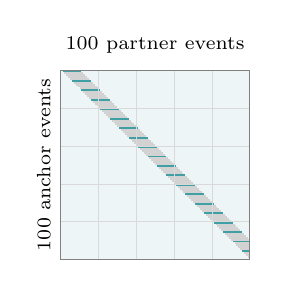
\begin{tikzpicture}[x=.024cm,y=.024cm,every node/.style={font=\scriptsize}]
 \fill[pale] (0,0) rectangle (100,-100);
 \foreach \row in {0,...,98} {
   \pgfmathtruncatemacro{\last}{min(100,\row+11)}
   \fill[gray!35] (\row+1,-\row) rectangle (\last,-\row-1);
 }
 \foreach \row in {0,5,...,95} {
 \pgfmathtruncatemacro{\last}{min(100,\row+11)}
 \fill[teal!75] (\row+1,-\row) rectangle (\last,-\row-1);
}
 \foreach \tick in {0,20,...,100} {
   \draw[gray!30,line width=.2pt] (\tick,0)--(\tick,-100);
   \draw[gray!30,line width=.2pt] (0,-\tick)--(100,-\tick);
 }
 \draw[gray] (0,0) rectangle (100,-100);
 \node[above] at (50,4) {100 partner events};
 \node[rotate=90] at (-9,-50) {100 anchor events};
\end{tikzpicture}
 \par\smallskip
 \textcolor{teal}{193 event pairs}\par
 \footnotesize Every fifth anchor window; skipped windows are grey.
 \end{column}
 \begin{column}{.47\textwidth}
 \centering\textbf{Depth 10, stride 1}\par\smallskip
 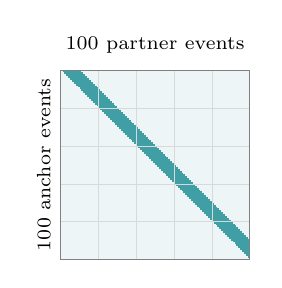
\begin{tikzpicture}[x=.024cm,y=.024cm,every node/.style={font=\scriptsize}]
 \fill[pale] (0,0) rectangle (100,-100);
 \foreach \row in {0,...,98} {
   \pgfmathtruncatemacro{\last}{min(100,\row+11)}
   \fill[teal!75] (\row+1,-\row) rectangle (\last,-\row-1);
 }
 
 \foreach \tick in {0,20,...,100} {
   \draw[gray!30,line width=.2pt] (\tick,0)--(\tick,-100);
   \draw[gray!30,line width=.2pt] (0,-\tick)--(100,-\tick);
 }
 \draw[gray] (0,0) rectangle (100,-100);
 \node[above] at (50,4) {100 partner events};
 \node[rotate=90] at (-9,-50) {100 anchor events};
\end{tikzpicture}
 \par\smallskip
 \textcolor{teal}{945 event pairs}\par
 \footnotesize Every anchor, with up to ten partner events.
 \end{column}
 \end{columns}
 \par\smallskip
 \footnotesize Mixing runs to the pool edge: the last anchor windows contain \textbf{fewer than 10 partner events}.\par\smallskip
 Stride 5 reduces event pairs by about 80\%. Events from different pools never mix.
 \note{Schematic selfCombinations ordering within one dataframe and pool. Depth 10 produces sum(min(10,99-i),i=0..98)=945 event pairs. Stride 5 retains anchor windows i=0,5,...,95, yielding 18*10+9+4=193 event pairs. Grey cells are eligible depth-10 event pairs whose anchor window is skipped. No individual events are labelled; coarse grid lines are visual guides every 20 events. Actual selection, field consistency and valid particle-pair acceptance can lower effective counts.}
 \src{O2Physics/PWGCF/Femto/Core/pairProcessHelpers.h; O2Physics/PWGCF/Femto/Core/pairHistManager.h}
\end{frame}

\begin{frame}[fragile]{Part 3: close-pair rejection}
 \begin{columns}[T]
 \begin{column}{.48\textwidth}
 \begin{lstlisting}
"CprTrackV0Daughter": {
  "cutAverage": "false",
  "cutAnyRadius": "true",
  "cutElipsoidal": "true",
  "detaMax": "0.01",
  "dphistarMax": "0.01",
  "detaCenter": "0",
  "dphistarCenter": "0"
}
 \end{lstlisting}
 \small For proton--$\Lambda$, the primary track is compared with the charged daughters.\par\medskip
 Both cut switches \texttt{"false"} disable CPR.
 \end{column}
 \begin{column}{.48\textwidth}
 \centering
 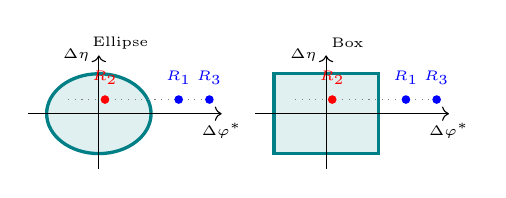
\begin{tikzpicture}[scale=.78,every node/.style={font=\tiny}]
 \foreach \offset/\shape in {0/Ellipse,1/Box} {
   \begin{scope}[shift={(3.7*\offset,0)}]
     \node at (.35,1.15) {\shape};
     \ifnum\offset=0\relax
       \fill[teal!12] (0,0) ellipse (.85 and .65);
       \draw[teal,very thick] (0,0) ellipse (.85 and .65);
     \else
       \fill[teal!12] (-.85,-.65) rectangle (.85,.65);
       \draw[teal,very thick] (-.85,-.65) rectangle (.85,.65);
     \fi
     \draw[->] (-1.15,0)--(2.0,0) node[below] {$\Delta\varphi^*$};
     \draw[->] (0,-.9)--(0,.95) node[left] {$\Delta\eta$};
     \draw[dotted,gray] (-.5,.23)--(1.8,.23);
     \fill[red] (.1,.23) circle (2pt) node[above=2pt] {$R_2$};
     \fill[blue] (1.3,.23) circle (2pt) node[above=2pt] {$R_1$};
     \fill[blue] (1.8,.23) circle (2pt) node[above=2pt] {$R_3$};
   \end{scope}
 }
 \end{tikzpicture}
 \par\smallskip
 \footnotesize One radius ($R_2$) lies inside the cut: \texttt{cutAnyRadius = true} rejects the pair.\par\medskip
 \texttt{cutAverage}: tests the average $\Delta\varphi^*$ over radii.\par\medskip
 \texttt{cutElipsoidal = true}: ellipse.\par
 \texttt{cutElipsoidal = false}: box.\par\smallskip
 The cut can be off-centre: set \texttt{detaCenter} and \texttt{dphistarCenter}.
 \end{column}
 \end{columns}
 \src{O2Physics/PWGCF/Femto/Core/closePairRejection.h}
\end{frame}

\begin{frame}{Part 3: all CPR diagnostic options}
 \footnotesize
 \renewcommand{\arraystretch}{1.08}
 \begin{tabular}{p{.42\textwidth}p{.52\textwidth}}
 \toprule
 \texttt{CprTrackV0Daughter} option & Purpose\\\midrule
 \texttt{plotAllRadii}, \texttt{plotAverage} & $\Delta\eta$--$\Delta\varphi^*$ at each radius / averaged.\\
 \texttt{plotAngularCorrelation} & $\eta_1$ vs $\eta_2$, $\varphi_1$ vs $\varphi_2$.\\
 \texttt{plotKinematic} & Distribution of blocked pairs.\\
 \texttt{kinematicVariable} & \texttt{"0"}: $k^*$, \texttt{"1"}: $k_{\rm T}$, \texttt{"2"}: $m_{\rm T}$, \texttt{"3"}: $Q_3$.\\
 \texttt{kinematicMin}, \texttt{kinematicMax} & Kinematic window for plotting; negative disables a bound.\\
 \texttt{binningKinematic} & Axis of blocked-pair kinematics.\\
 \texttt{binningDeta}, \texttt{binningDphistar} & Close-pair QA axes.\\
 \texttt{binningCorrelationPhi}, \texttt{binningCorrelationEta} & Angular-correlation QA axes.\\
 \texttt{seed} & Role randomization: negative off, zero time-based, positive fixed.\\
 \texttt{magField} & Field in kG for pure generator-level MC; reco uses collision field.\\\bottomrule
 \end{tabular}
 \src{O2Physics/PWGCF/Femto/Core/closePairRejection.h}
\end{frame}

\begin{frame}[fragile]{Part 3: pair cleaning and pair cuts}
 \begin{block}{A track cannot be paired with its own $\Lambda$}
 The cleaner rejects a primary-track candidate when its stored track index matches either $\Lambda$ daughter index. This check is automatic; there is no activation flag for shared-track cleaning.
 \end{block}
 \begin{columns}[T]
 \begin{column}{.48\textwidth}
 \begin{lstlisting}
"PairCuts": {
  "kstarMin": "-1", "kstarMax": "-1",
  "ktMin": "-1", "ktMax": "-1",
  "mtMin": "-1", "mtMax": "-1",
  "massInvMin": "-1", "massInvMax": "-1",
  "mixOnlyCommonAncestor": "false",
  "mixOnlyNonCommonAncestor": "false",
  "useMotherAsAncestor": "false",
  "kinematicVariable": "0"
}
 \end{lstlisting}
 \end{column}
 \begin{column}{.48\textwidth}
 \small Negative pair-kinematic bounds are disabled.\par\medskip
 In MC, ancestry can require common or non-common ancestry (mutually exclusive); \texttt{useMotherAsAncestor} chooses direct mother instead of partonic mother.\par\medskip
 \texttt{PairCuts.kinematicVariable} selects the kinematic variable: $k^*$, $k_{\rm T}$ or $m_{\rm T}$.\par\smallskip
 \texttt{PairCleanerBinning.kinematic} sets its histogram binning for blocked pairs.
 \end{column}
 \end{columns}
 \src{O2Physics/PWGCF/Femto/Core/pairCleaner.h; O2Physics/PWGCF/Femto/Core/pairHistManager.h}
\end{frame}

\begin{frame}[fragile]{Part 3: which ancestor is compared?}
 \begin{lstlisting}
"femto-producer": {
  "MonteCarlo": {"findLastPartonicMother": "true"}
}
 \end{lstlisting}
 \begin{itemize}
 \item \texttt{true}: first parton after the initial collision, before reaching a beam particle when tracing backwards.
 \item \texttt{false}: last parton before hadronization, closest to the final-state hadron.
 \end{itemize}
 \begin{block}{Producer choice, consumer comparison}
 \small The producer stores the chosen partonic ancestor. With \texttt{useMotherAsAncestor = false}, common/non-common checks compare these stored ancestors.\par\smallskip
 \texttt{useMotherAsAncestor = true} instead compares the direct mothers.
 \end{block}
 \note{The findLastPartonicMother name refers to backwards traversal: true follows the ancestry back towards the beam and retains the earliest parton after the initial collision. False selects the nearest partonic ancestor before hadronization. Both choices are partons, not a hadron before hadronization. The setting belongs to the producer MonteCarlo group and cannot be changed retrospectively by a consumer reading derived MC tables. Common and non-common requirements remain mutually exclusive.}
 \src{O2Physics/PWGCF/Femto/Core/mcBuilder.h; O2Physics/PWGCF/Femto/Core/pairCleaner.h}
\end{frame}



\begin{frame}{Part 3: mixing without collision tagging}
 \centering
 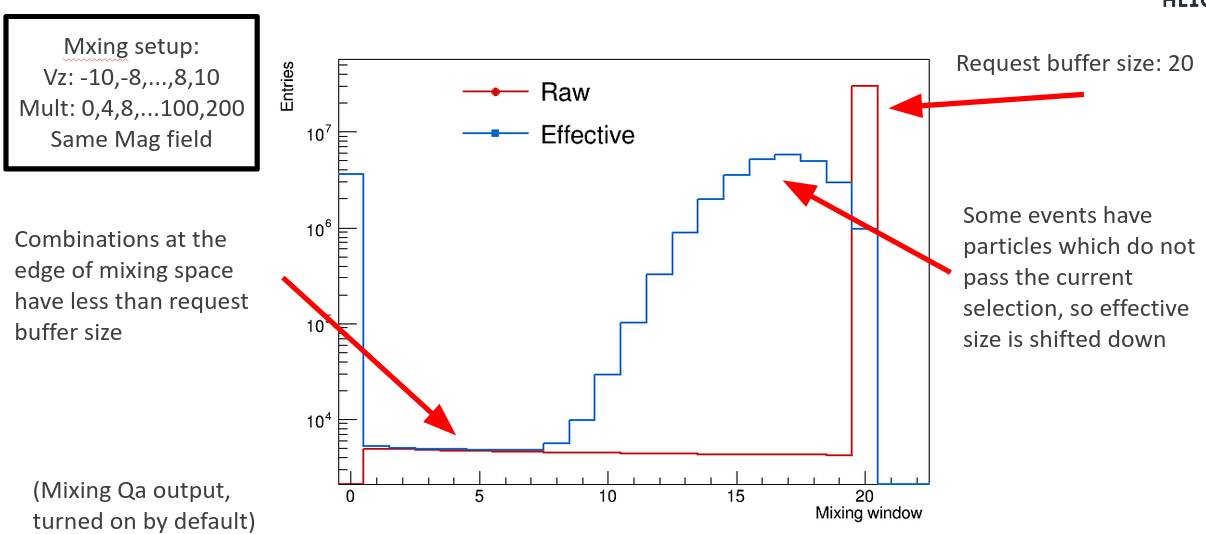
\includegraphics[width=\textwidth,height=.76\textheight,keepaspectratio]{slides/assets/mixing-without-tagging.png}
 \note{User-provided screenshot from another presentation. Raw windows reach the requested depth, apart from boundaries; effective windows lose partners without suitable selected candidates. The screenshot's statement that mixing QA is on by default refers to its original setup: in this checkout enableEventMixingQa defaults to false, and our demonstration explicitly enables it.}
 \src{O2Physics/PWGCF/Femto/Core/pairHistManager.h; O2Physics/PWGCF/Femto/Core/pairProcessHelpers.h}
\end{frame}

\begin{frame}{Part 3: mixing with collision tagging}
 \centering
 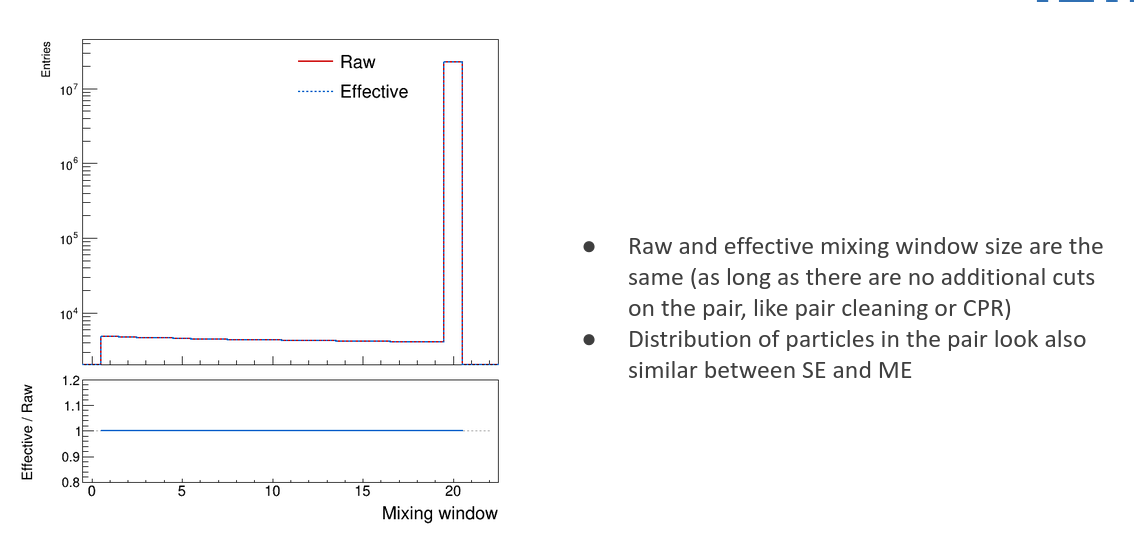
\includegraphics[width=\textwidth,height=.76\textheight,keepaspectratio]{slides/assets/mixing-with-tagging.png}
 \note{User-provided screenshot from another presentation. Tagging retains collisions containing the configured candidate species, so raw and effective mixing-window sizes can agree. Subsequent pair cleaning, CPR and pair cuts can still remove every candidate pair for a partner event, reducing the effective window. The screenshot is illustrative, not an output generated by the tutorial scripts.}
 \src{O2Physics/PWGCF/Femto/TableProducer/femtoProducerCollisionTagger.cxx; O2Physics/PWGCF/Femto/Core/pairProcessHelpers.h}
\end{frame}

\begin{frame}[fragile]{Part 3: pair histograms and dimensions}
 \begin{columns}[T]
 \begin{column}{.43\textwidth}
 \begin{lstlisting}[basicstyle=\ttfamily\fontsize{7}{8}\selectfont]
femto-pair-track-v0/
  TrackV0/
    SE/Analysis/...
    ME/Analysis/...
  TrackV0Cleaner/
    SE/...
    ME/...
  CPR_TrackV0Dau/
    SE/...
    ME/...
 \end{lstlisting}
 \small Same- and mixed-event pair distributions, shared-track cleaning and close-pair rejection QA.
 \end{column}
 \begin{column}{.53\textwidth}
 \begin{lstlisting}[basicstyle=\ttfamily\fontsize{7}{8}\selectfont]
"PairBinning": {
  "plotKstarVsMtVsMult": "false",
  "plotKstarVsMtVsMultVsCent": "true",
  "kstar": {"values": ["600", "0", "6"]},
  "mt": {"values": ["100", "1", "6"]},
  "multiplicity": {"values": ["1", "0", "5000"]},
  "centrality": {"values": ["1", "0", "100"]}
}
 \end{lstlisting}
 \small Plot switches turn higher-dimensional histograms on or off.
 \end{column}
 \end{columns}
 \par
 \small\textbf{Reuse a higher-dimensional THnSparse:} set unused dimensions to one bin covering their full range. No extra bin multiplicity in these axes; no separate histogram implementation for every axis combination.
 \note{The example enables hKstarVsMtVsMultVsCent and makes multiplicity and centrality inclusive via one bin, leaving differential kstar and mt axes. Use ranges covering the complete selected sample and handle underflow/overflow consistently in projections. Higher-dimensional sparse histograms allocate populated bins rather than the full Cartesian grid. Extra axes still have small coordinate/metadata overhead, so this is not a claim of literally zero memory/CPU cost. Basic 1D/2D pair histograms are TH1F/TH2F, not THnSparse; the reuse argument here applies to the higher-dimensional THnSparse plots. The histogram choices shown are illustrative and do not alter the runnable baseline configuration.}
 \src{O2Physics/PWGCF/Femto/Core/pairHistManager.h; O2Physics/PWGCF/Femto/Core/pairCleaner.h; O2Physics/PWGCF/Femto/Core/closePairRejection.h}
\end{frame}

\begin{frame}[fragile]{Part 3: single-particle histograms in the pair task}
 \begin{lstlisting}
femto-pair-track-v0/
  Track1/SE/Analysis/...     Track1/ME/Analysis/...
  Lambda1/SE/Analysis/...    Lambda1/ME/Analysis/...
 \end{lstlisting}
 \begin{columns}[T]
 \begin{column}{.48\textwidth}
 \begin{block}{Same event (SE)}
 \small Filled only when the collision contributes at least one valid pair.\par\medskip
 Each selected particle is filled \textbf{once per collision}, even if the collision contains several valid pairs.
 \end{block}
 \end{column}
 \begin{column}{.48\textwidth}
 \begin{block}{Mixed event (ME)}
 \small Filled for every valid mixed-event pair.\par\medskip
 A particle is filled \textbf{as many times as it is used} in accepted mixed-event pairs.
 \end{block}
 \end{column}
 \end{columns}
 \medskip
 \small SE and ME therefore retain their different particle-sampling weights.
 \note{Valid means after particle cleaning, shared-track pair cleaning, CPR and pair cuts. For SE, once any pair is accepted, the task loops over the selected particle slices and fills each particle that passes the particle cleaner once. Thus the SE constituent sample includes all selected cleaner-passing particles in a contributing collision, not only the unique constituents of accepted pairs. ME fills constituents inside the accepted-pair loop, so repeated uses carry repeated weight. The same distinction applies to single-particle FitVars histograms discussed later. Run scripts and local/Hyperloop instructions remain in the example directory for the live demonstration.}
 \src{O2Physics/PWGCF/Femto/Core/pairProcessHelpers.h; O2Physics/PWGCF/Femto/Core/pairBuilder.h}
\end{frame}

\section{Example 2: studying cuts with pass-through production}

\begin{frame}[fragile]{Example 2: passthrough mode}
 \footnotesize
 \begin{lstlisting}
 "TrackBits": {
   "passThrough": "true"
 }
 \end{lstlisting}
 \begin{itemize}
 \item All track selections become non-mandatory: decisions are stored, but no track is discarded by them.
 \item Track filter options are ignored for acceptance; no track is discarded by the filters either.
 \item Every configured decision is stored, including the loosest threshold bits.
 \item QA consumers reproduce the before/after-cut workflow commonly used in Run 2.
 \end{itemize}
 \begin{block}{Each wagon sees the same input}
 Baseline $\to$ add TPC clusters $\to$ add crossed rows $\to$ add ITS clusters $\to$ add proton PID.
 \end{block}
 \small Changing the selection type changes the bit mapping: \textbf{recompute the consumer bitmasks with CutCulator} using the passthrough producer output. Collision selections are unchanged here.
 \note{In the current local implementation checkFilters returns isPassThrough() || pass, so track prefilters are evaluated for QA but do not reject tracks. BaseSelection makes configured track decisions neutral, stores the loosest bits and bypasses bit-based acceptance; they are not optional acceptance gates in this mode. CollisionBits.passThrough is separate and stays false. The baseline has no additional track cuts but still shares the collision sample and input reconstruction acceptance.}
 \src{O2Physics/PWGCF/Femto/Core/trackBuilder.h; O2Physics/PWGCF/Femto/Core/baseSelection.h}
\end{frame}

\begin{frame}[fragile]{Example 2: independent QA wagons in one chain}
 \begin{lstlisting}[language=bash]
 o2-analysis-cf-femto-producer "${Options[@]}" |
 o2-analysis-cf-femto-track-qa "${Options[@]}" --workflow-suffix -base |
 o2-analysis-cf-femto-track-qa "${Options[@]}" --workflow-suffix -clusters |
 o2-analysis-cf-femto-track-qa "${Options[@]}" --workflow-suffix -rows |
 o2-analysis-cf-femto-track-qa "${Options[@]}" --workflow-suffix -its |
 o2-analysis-cf-femto-track-qa "${Options[@]}" --workflow-suffix -pid |
 # ... the same helper tasks as in Example 1
 \end{lstlisting}
 \small Each suffix creates a separate task and ROOT output directory.\par
 Configuration keys match the names, e.g.\par
 \texttt{"femto-track-qa-rows": \{ "TrackSelection1": ... \}}.
 \medskip
 \textbf{The cuts are cumulative in the masks, not in task order.} Every wagon reads the producer tables directly.
 \note{The full executable pipeline is in examples/02-cut-study/run.sh. The displayed pipe is an excerpt. workflow-suffix is applied to each QA executable independently; do not set it globally on the common options. All wagons use the same histogram settings, collision filter and broad track kinematics.}
 \src{O2Physics/PWGCF/Femto/Tasks/femtoTrackQa.cxx}
\end{frame}

\begin{frame}{Example 2: cumulative selections}
 \small \texttt{examples/02-cut-study/configuration.json}
 \medskip
 \renewcommand{\arraystretch}{1.3}
 \begin{tabular}{llcc}
 \toprule
 Wagon & Newly added cut & Low-$p$ mask & High-$p$ mask\\
 \midrule
 \texttt{base} & None & \texttt{"0"} & \texttt{"0"}\\
 \texttt{clusters} & TPC clusters $\geq90$ & \texttt{"1"} & \texttt{"1"}\\
 \texttt{rows} & Crossed rows $\geq100$ & \texttt{"17"} & \texttt{"17"}\\
 \texttt{its} & ITS clusters $\geq5$ & \texttt{"529"} & \texttt{"529"}\\
 \texttt{pid} & Proton PID & \texttt{"33297"} & \texttt{"131601"}\\
 \bottomrule
 \end{tabular}
 \medskip
 Each row retains the previous requirements and adds one more decision.
 \begin{block}{The incremental effect of each cut}
 Each wagon has its own QA distributions and retained track count. Differences relative to the preceding wagon show the incremental effect in this cut order.
 \end{block}
 \note{These masks were verified against initialization metadata for this pass-through configuration. Individual bits are TPC clusters >=90: 1, crossed rows >=100: 16, ITS clusters >=5: 512, TPC proton PID: 32768, combined TPCTOF proton PID: 131072. The latter two are used below/above pidThres=0.75 respectively. All track signs are kept. This is an ordered cut study, not a claim of independent per-cut efficiencies.}
 \src{O2Physics/PWGCF/Femto/Core/partitions.h; O2Physics/PWGCF/Femto/Tasks/femtoTrackQa.cxx}
\end{frame}

\begin{frame}[fragile]{Example 2: QA comparison}
 \begin{lstlisting}[language=bash]
 bash examples/02-cut-study/run.sh
 \end{lstlisting}
 \begin{itemize}
 \item The same root-level AO2D is referenced by \texttt{input\_data.txt}.
 \item Output: \texttt{examples/02-cut-study/AnalysisResults.root}.
 \item Separate outputs: \texttt{femto-track-qa-base}, \texttt{-clusters}, \texttt{-rows}, \texttt{-its} and \texttt{-pid}.
 \end{itemize}
 \medskip
 \textbf{On Hyperloop:} the equivalent workflow has one pass-through producer and five uniquely named QA wagons with the same cumulative masks and separate outputs.
 \note{Two-dimensional plots are disabled in this example to keep the repeated QA output small. Enable the same plot options in all wagons if more detailed PID studies are needed.}
 \src{O2Physics/PWGCF/Femto/Tasks/femtoTrackQa.cxx}
\end{frame}

\section{Derived data}

\begin{frame}{Example 3: produce once, analyse many times}
 \small
 {\centering
 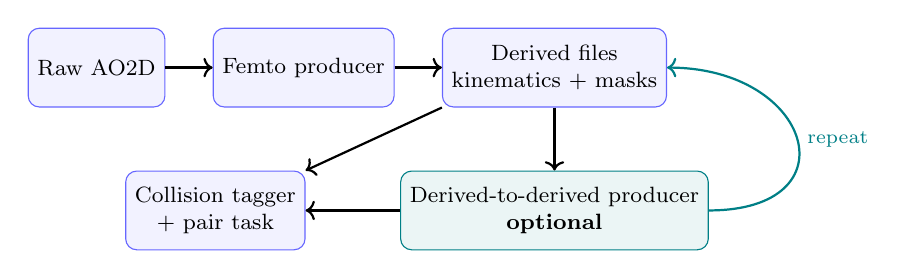
\begin{tikzpicture}[node distance=6mm,every node/.style={align=center,font=\footnotesize},box/.style={draw=blue!60,fill=blue!5,rounded corners,minimum height=10mm}]
 \node[box] (raw) {Raw AO2D};
 \node[box,right=of raw] (prod) {Femto producer};
 \node[box,right=of prod] (derived) {Derived files\\kinematics + masks};
 \node[box,below=8mm of derived,draw=teal,fill=teal!8] (d2d) {Derived-to-derived producer\\\textbf{optional}};
 \draw[->,thick] (raw)--(prod);
 \draw[->,thick] (prod)--(derived);
 \draw[->,thick] (derived)--(d2d);
 \draw[->,thick,teal] (d2d.east) to[out=0,in=0,looseness=2.5] node[right,font=\scriptsize] {repeat} (derived.east);
 \node[box,left=12mm of d2d] (pairs) {Collision tagger\\+ pair task};
 \draw[->,thick] (derived.south west)--(pairs.north east);
 \draw[->,thick] (d2d)--(pairs);
 \end{tikzpicture}\par}
 \medskip
 \begin{itemize}
 \item Producer-only workflow: raw AO2D dependencies, without QA or pairing.
 \item Standalone analysis: the derived tables already contain the required information.
 \item The optional derived-to-derived producer can run repeatedly on the derived files, refining the stored sample.
 \end{itemize}
 \src{O2Physics/PWGCF/Femto/TableProducer/femtoProducer.cxx; O2Physics/PWGCF/Femto/DataModel/FemtoTables.h}
\end{frame}

\begin{frame}[fragile]{Derived production: explicitly enable the output tables}
 \begin{lstlisting}
"CollisionTables": {
  "produceCollisions": "1", "produceCollisionMasks": "1"
},
"TrackTables": {
  "produceTracks": "1", "produceTrackMasks": "1"
},
"V0Tables": {
  "produceLambdas": "1", "produceLambdaMasks": "1"
}
 \end{lstlisting}
 \begin{itemize}
 \item \texttt{"-1"}: auto-enable from downstream task subscriptions in a full workflow.
 \item \texttt{"1"}: force on for a producer-only derived-data production; \texttt{"0"}: force off.
 \item Only kinematics and masks are stored: the QA tasks cannot run on this derived dataset.
 \end{itemize}
 \note{Additional extra-observable tables could be stored to enable QA, but they are intentionally omitted from this compact example. All unrelated table switches are explicitly off in producer.json. Do not delete daughter-only track rows: Lambda daughter references must remain valid for the cleaner and CPR. Keep AnalysisResults.root with the producer configuration/selection metadata alongside the derived file; the minimal six-table output does not contain detector observables or that histogram metadata.}
 \src{O2Physics/PWGCF/Femto/Core/trackBuilder.h; O2Physics/PWGCF/Femto/Core/v0Builder.h; O2Physics/PWGCF/Femto/Core/collisionBuilder.h}
\end{frame}

\begin{frame}[fragile]{Derived production: the writer selects what reaches disk}
 \begin{lstlisting}
{
  "OutputDirector": {
    "resfile": "FemtoDerived", "resfilemode": "RECREATE",
    "OutputDescriptors": [
      {"table": "AOD/FCOL/1"}, {"table": "AOD/FCOLMASK/1"},
      {"table": "AOD/FTRACK/1"}, {"table": "AOD/FTRACKMASK/1"},
      {"table": "AOD/FLAMBDA/1"}, {"table": "AOD/FLAMBDAMASK/2"}
    ]
  }
}
 \end{lstlisting}
 \small \texttt{--aod-writer-json writer.json} activates this output selection.\par\medskip
 \texttt{examples/03-derived-data/produce.sh} runs the producer and its raw-AO2D dependencies.\par\medskip
 Two outputs: \texttt{FemtoDerived.root} (tables) and \texttt{AnalysisResults.root} (producer metadata).
 \note{The table descriptor includes origin, description and version; these match the local FemtoTables.h. The writer configuration is separate from DPL task configuration. The default one-timeframe-per-output-DF behavior is retained. OutputDirector ntfmerge is intentionally omitted: unlike task configurable values, its JSON parser requires a numeric JSON value.}
 \src{O2Physics/PWGCF/Femto/DataModel/FemtoTables.h; O2/Framework/Core/src/DataOutputDirector.cxx}
\end{frame}

\begin{frame}{Hyperloop: producer wagon and derived-data output}
 \centering
 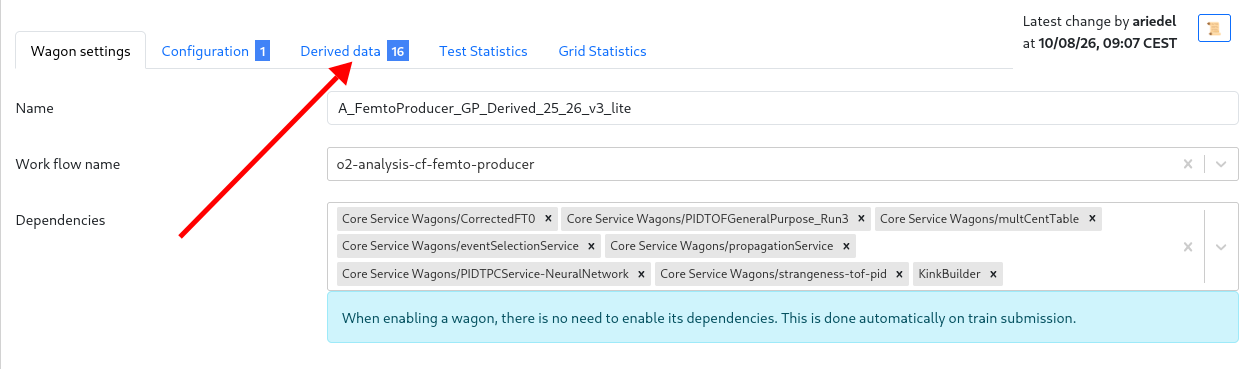
\includegraphics[width=\textwidth,height=.66\textheight,keepaspectratio]{slides/assets/hyperloop-producer-wagon.png}
 \par\medskip
 \small The producer wagon's \textbf{Derived data} tab configures which output tables are written.
 \note{User-provided screenshot. The dependency list shown belongs to this example wagon and includes additional species beyond the proton-Lambda tutorial. Hyperloop automatically includes configured dependencies on train submission, as indicated in the UI.}
 \src{O2Physics/PWGCF/Femto/TableProducer/femtoProducer.cxx}
\end{frame}

\begin{frame}{Hyperloop: select the derived tables}
 \centering
 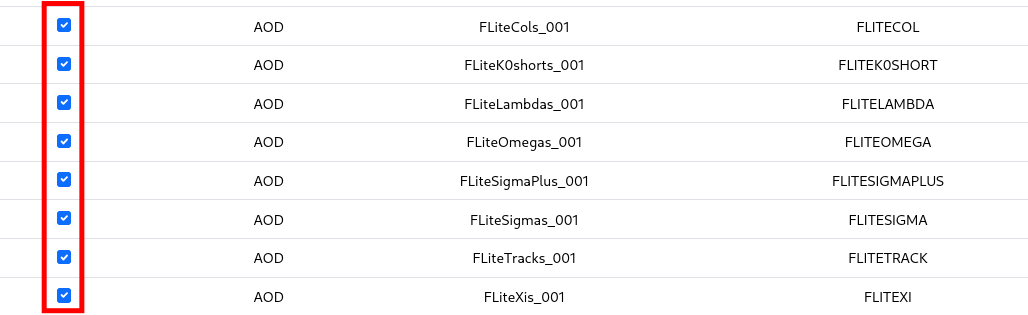
\includegraphics[width=\textwidth,height=.66\textheight,keepaspectratio]{slides/assets/hyperloop-derived-tables.png}
 \par\medskip
 \small Select the tables to write; a Lite-table production is shown here.
 \note{User-provided screenshot illustrating table checkboxes. This screenshot contains multiple Lite species; the local tutorial instead writes the full-kinematic collision, track and Lambda tables with their masks. Select the table set appropriate to the production and downstream consumers; do not treat the screenshot as the exact six-table tutorial selection.}
 \src{O2Physics/PWGCF/Femto/DataModel/FemtoTables.h}
\end{frame}

\begin{frame}{Hyperloop: force the selected producer tables on}
 \centering
 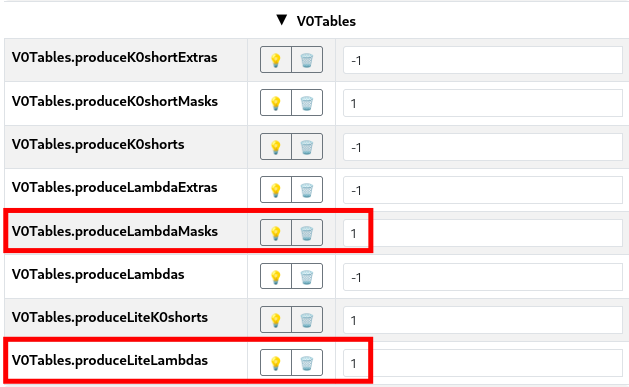
\includegraphics[width=.78\textwidth,height=.70\textheight,keepaspectratio]{slides/assets/hyperloop-producer-table-flags.png}
 \par\smallskip
 \small Selected output tables must also be produced: set their producer switches to \texttt{1}.
 \note{User-provided screenshot of V0Tables. The highlighted example forces Lambda masks and Lite Lambdas on. Auto mode -1 follows downstream subscriptions; for producer-only output, explicitly enabling the intended tables avoids depending on consumer task subscriptions. Writer selection and producer table enablement are separate settings.}
 \src{O2Physics/PWGCF/Femto/Core/v0Builder.h}
\end{frame}

\begin{frame}[fragile]{Standalone pairing on derived data}
 \small
 \begin{lstlisting}[language=bash]
# examples/03-derived-data/analyze.sh
# input_derived.txt contains: FemtoDerived.root
Options=(-b --configuration json://pair.json
         --aod-file @input_derived.txt)
o2-analysis-cf-femto-producer-collision-tagger "${Options[@]}" |
  o2-analysis-cf-femto-pair-track-v0 "${Options[@]}" --run
 \end{lstlisting}
 \begin{itemize}
 \item The same \texttt{TrackSelection1}, \texttt{LambdaSelection1}, mixing and pair settings.
 \item Collision tagging is included from the start and recomputed for the current pair wagon.
 \item Raw-AO2D event-selection, propagation and PID services are no longer needed.
 \end{itemize}
 \small Local: derived input list + \texttt{pair.json}.\par
 Hyperloop: derived dataset + tagger and pair wagons; matching table versions.
 \src{O2Physics/PWGCF/Femto/Tasks/femtoPairTrackV0.cxx; O2Physics/PWGCF/Femto/TableProducer/femtoProducerCollisionTagger.cxx}
\end{frame}

\begin{frame}[fragile]{Local dataframe sizes: \texttt{o2-aod-merger}}
 \begin{lstlisting}[language=bash]
o2-aod-merger --input input_derived.txt \
  --output FemtoMerged.root --max-size 100000000
 \end{lstlisting}
 \begin{itemize}
 \item Input: a text list of compatible, self-contained derived ROOT files.
 \item Combines complete input dataframes into larger output \texttt{DF\_...} directories and updates table indices.
 \item \texttt{--max-size}: approximate target size of an uncompressed dataframe directory, in bytes; it is not a ROOT file-size limit.
 \item Larger dataframes can provide more mixing partners; they also require more memory.
 \end{itemize}
 \begin{block}{Boundary of the operation}
 An existing large dataframe is not split into smaller ones. \texttt{--max-size 0} preserves input dataframe boundaries (needed for non-self-contained inputs).
 \end{block}
 \note{The size is tested after copying a whole input DF, so the target can be exceeded. Do not use hadd for AOD tables with row-index references. The example merge.sh refuses to overwrite an existing output. No merger is needed to combine histogram-only AnalysisResults.root files.}
 \src{O2/Framework/AODMerger/src/aodMerger.cxx}
\end{frame}

\section{Derived-to-derived production}

\begin{frame}{Derived-to-derived: make a smaller analysis dataset}
 \centering
 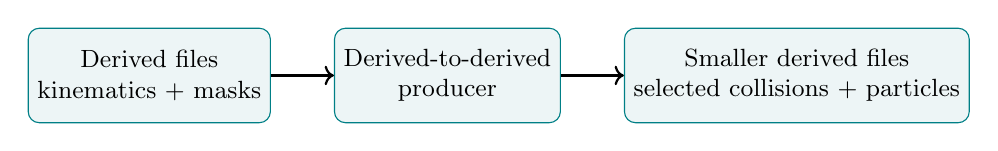
\begin{tikzpicture}[node distance=8mm,every node/.style={align=center,font=\small},box/.style={draw=teal,fill=pale,rounded corners,minimum height=12mm}]
 \node[box] (input) {Derived files\\kinematics + masks};
 \node[box,right=of input] (skim) {Derived-to-derived\\producer};
 \node[box,right=of skim] (output) {Smaller derived files\\selected collisions + particles};
 \draw[->,thick] (input)--(skim);\draw[->,thick] (skim)--(output);
 \end{tikzpicture}\par
 \medskip
 \begin{itemize}
 \item Applies consumer-style kinematic selections and masks to existing derived tables.
 \item Keeps collisions with enough selected candidates; optionally downsamples them.
 \item Rewrites collision and daughter indices while preserving the stored masks.
 \item Can run again on its own output. Previously discarded information cannot be recovered.
 \end{itemize}
 \note{This task does not repeat detector PID or quality evaluation and does not create new threshold decisions. It uses stored kinematics and masks. Daughter tracks are copied as needed even if they do not pass the standalone-track selection, with deduplication and reference remapping. Subsequent consumers still use their particle partitions. Unlike collision tagging, which supplies a selection-dependent tag to mixing, this task creates a persistently smaller dataset.}
 \src{O2Physics/PWGCF/Femto/TableProducer/femtoProducerDerivedToDerived.cxx; O2Physics/PWGCF/Femto/Core/trackBuilder.h}
\end{frame}

\begin{frame}[fragile]{Derived-to-derived: familiar particle selections}
 \begin{lstlisting}
"CollisionSelection": {"vtxZMin": "-10", "vtxZMax": "10"},
"TrackSelection1": {
  "pdgCodeAbs": "2212", "chargeSign": "0", "chargeAbs": "1",
  "ptMin": "0.3", "ptMax": "4", "pidThres": "0.75",
  "maskLowMomentum": "64", "maskHighMomentum": "256"
},
"LambdaSelection1": {
  "pdgCodeAbs": "3122", "sign": "1", "mask": "15",
  "massMin": "1.11", "massMax": "1.12"
}
 \end{lstlisting}
 \begin{itemize}
 \item The same configurable groups used by QA and pair consumers.
 \item \texttt{chargeSign = 0} keeps both track charges for later analyses.
 \item Masks refer to the original producer's bit mapping; skimming preserves that mapping.
 \end{itemize}
 \note{These values match the normal-production proton-Lambda example. Masks must instead be computed from the matching metadata for a Hyperloop dataset or passthrough input. The full example JSON carries all kinematic bounds from the pair configuration. Lambda sign 1 keeps Lambda; sign 0 can retain both Lambda and anti-Lambda when the mask selection is appropriate for the supplied production. Keeping both track charges does not mean every retained track will pass a subsequent positive-proton partition.}
 \src{O2Physics/PWGCF/Femto/Core/partitions.h; O2Physics/PWGCF/Femto/TableProducer/femtoProducerDerivedToDerived.cxx}
\end{frame}

\begin{frame}[fragile]{Derived-to-derived: candidate counts and downsampling}
 \begin{lstlisting}
"TrackTables": {"limitTrack1": "1", "limitTrack2": "0"},
"V0Tables": {"limitLambda": "1", "limitK0short": "0"},
"CollisionDownsampling": {"fraction": "1", "seed": "42"}
 \end{lstlisting}
 \begin{itemize}
 \item This example requires at least one selected track and one selected $\Lambda$ per collision.
 \item A limit of \texttt{0} disables that candidate category: it is neither required nor written as a standalone species.
 \item \texttt{fraction = 1} keeps all surviving collisions; \texttt{0.1} randomly keeps 10\%.
 \item A fixed positive seed gives reproducible downsampling; \texttt{0} chooses a time-based seed.
 \end{itemize}
 \begin{block}{Daughter references remain valid}
 \small Required $\Lambda$ daughters are retained in the track table, even when they fail the standalone-track selection.
 \end{block}
 \note{Counts are checked on the configured partitions before downsampling and writing. A track category limit 0 does not prevent a composite-particle builder from copying a necessary daughter track. Overlapping track selections and daughter reuse are deduplicated in the output. A sample conditioned on candidate counts has a different collision population from the original production, relevant when interpreting event-normalized quantities and mixing.}
 \src{O2Physics/PWGCF/Femto/Core/trackBuilder.h; O2Physics/PWGCF/Femto/Core/v0Builder.h; O2Physics/PWGCF/Femto/Core/collisionBuilder.h}
\end{frame}

\begin{frame}[fragile]{Derived-to-derived: choose the input subscription}
 \begin{lstlisting}
"femto-producer-derived-to-derived": {
  "processTracks": "false",
  "processTracksLambdas": "true"
}
 \end{lstlisting}
 \begin{itemize}
 \item Exactly one process function is enabled; its arguments define the required input tables.
 \item \texttt{processTracksLambdas}: collision, track and $\Lambda$ tables with masks.
 \item \texttt{processTracksLambdasWithFitVars}: additionally carries packed track PID, DCA and $\Lambda$ fraction variables.
 \item MC variants additionally need the corresponding truth and label tables.
 \end{itemize}
 \small A process cannot preserve observables that were not stored in the input production.
 \note{The default processTracks is true, so explicitly disabling it is essential when enabling processTracksLambdas. For reconstructed MC with FitVars the matching process is processTracksLambdasMcWithFitVars. The compact six-table data production supports the ordinary process only. No raw-AO2D event-selection, propagation or PID service belongs in this derived-only workflow.}
 \src{O2Physics/PWGCF/Femto/TableProducer/femtoProducerDerivedToDerived.cxx}
\end{frame}

\begin{frame}[fragile]{Derived-to-derived: select the rewritten output}
 \begin{lstlisting}
"OutputDirector": {
  "resfile": "FemtoSkim", "resfilemode": "RECREATE",
  "OutputDescriptors": [
    {"table": "AOD1/FCOL/1"}, {"table": "AOD1/FCOLMASK/1"},
    {"table": "AOD1/FTRACK/1"}, {"table": "AOD1/FTRACKMASK/1"},
    {"table": "AOD1/FLAMBDA/1"}, {"table": "AOD1/FLAMBDAMASK/2"}
  ]
}
 \end{lstlisting}
 \begin{itemize}
 \item The rewritten tables use the \texttt{AOD1} output stage, separating them from the \texttt{AOD} input tables in the workflow.
 \item The resulting file is read as derived input by the usual consumers or by another derived-to-derived pass.
 \item Collision tagging is recomputed in the analysis workflow for its current selections.
 \end{itemize}
 \note{writer.json is local DPL output selection, not DPL task configuration. It must select AOD1 to persist the rewritten tables rather than the original AOD input. The underlying stored table descriptions and versions match the ordinary full-kinematic tables, and the AOD reader exposes the persisted tables to downstream AOD consumers. Hyperloop's derived-data tab must likewise select the task's rewritten outputs.}
 \src{O2Physics/PWGCF/Femto/DataModel/FemtoTables.h; O2Physics/PWGCF/Femto/Core/v0Builder.h}
\end{frame}

\begin{frame}[fragile]{Derived-to-derived: Hyperloop first, then local}
 \begin{itemize}
 \item Hyperloop wagon: \texttt{o2-analysis-cf-femto-producer-derived-to-derived}, using the existing derived dataset as input.
 \item Configure selections, candidate limits and the process function; select the rewritten output tables.
 \item Download the configuration as \texttt{configuration.json} for the matching local workflow.
 \end{itemize}
 \begin{lstlisting}[language=bash]
# examples/05-derived-to-derived/
# input_data.txt: path to a downloaded derived ROOT file
bash examples/05-derived-to-derived/run.sh
 \end{lstlisting}
 \small The self-contained run script uses \texttt{configuration.json} and \texttt{writer.json}; output is \texttt{FemtoSkim.root}. A later pass can use that file as its input.
 \note{The script changes into its own directory. CONFIG_FILE and INPUT_DATA_FILE can override the defaults. It invokes only the derived-to-derived executable, with the local writer configuration. Input defaults to the output of the earlier compact derived-data example. Downloaded task configuration must match the producer metadata and table versions of the chosen dataset. --dry-run dumps the workflow without processing.}
 \src{O2Physics/PWGCF/Femto/TableProducer/femtoProducerDerivedToDerived.cxx}
\end{frame}

\begin{frame}{Derived-to-derived: four proton--$\Lambda$ datasets}
 \centering
 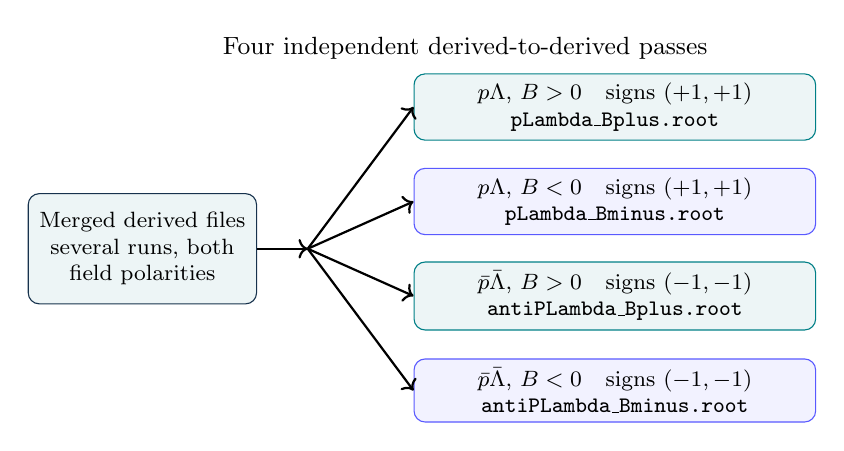
\begin{tikzpicture}[every node/.style={align=center,font=\footnotesize},outputbox/.style={draw=teal,fill=pale,rounded corners,minimum width=51mm,minimum height=8mm}]
 \node[draw=navy,fill=pale,rounded corners,minimum width=29mm,minimum height=14mm] (input) at (0,0) {Merged derived files\\several runs, both\\field polarities};
 \coordinate (split) at (2.1,0);
 \node[font=\small] at (4.1,2.55) {Four independent derived-to-derived passes};
 \node[outputbox] (pp) at (6,1.8) {$p\Lambda$, $B>0$\quad signs $(+1,+1)$\\\texttt{pLambda\_Bplus.root}};
 \node[outputbox,draw=blue!65,fill=blue!5] (pm) at (6,.6) {$p\Lambda$, $B<0$\quad signs $(+1,+1)$\\\texttt{pLambda\_Bminus.root}};
 \node[outputbox] (ap) at (6,-.6) {$\bar p\bar\Lambda$, $B>0$\quad signs $(-1,-1)$\\\texttt{antiPLambda\_Bplus.root}};
 \node[outputbox,draw=blue!65,fill=blue!5] (am) at (6,-1.8) {$\bar p\bar\Lambda$, $B<0$\quad signs $(-1,-1)$\\\texttt{antiPLambda\_Bminus.root}};
 \draw[->,thick] (input)--(split);
 \foreach \target in {pp,pm,ap,am} {\draw[->,thick] (split)--(\target.west);}
 \end{tikzpicture}\par
 \footnotesize Signs: \texttt{TrackSelection1.chargeSign}, \texttt{LambdaSelection1.sign}.\par
 Field selection: \texttt{CollisionSelection.magFieldMin / magFieldMax}.\par\smallskip
 Merging across runs can put different magnetic-field polarities in the same file; these four outputs keep the analysis samples separate.
 \note{Each box represents a separate configured production/pass, not four instances writing identical AOD1 tables in one workflow. For positive field use e.g. magFieldMin 0 and magFieldMax 10 kG, and for negative field -10 and 0; bounds must cover the fields of the chosen input. Positive/negative particle selections use chargeSign +1/-1 and Lambda sign +1/-1, with positive absolute PDG codes. Particle and antiparticle masks must be valid for their respective producer selections; do not assume one numerical Lambda mask describes both hypotheses in every production. Give each pass a separate writer resfile or output directory. A file boundary or merged run is not itself a field selection. The pair task also checks field consistency between mixed events; explicit splitting organizes the dataset and avoids spending mixing windows on incompatible polarities.}
 \src{O2Physics/PWGCF/Femto/TableProducer/femtoProducerDerivedToDerived.cxx; O2Physics/PWGCF/Femto/Core/partitions.h}
\end{frame}

\section{MC and reconstruction}

\begin{frame}[fragile]{Example 4: reconstructed particles with MC truth}
 \begin{lstlisting}
"femto-producer": {
  "processTracksV0sRun3pp": "false",
  "processTracksV0sRun3ppMc": "true",
  "CollisionBits": {"rctFlags": "0", "sel8": "1"}
},
"femto-track-qa": {"processData": "false", "processMc": "true"},
"femto-v0-qa": {"processLambda": "false", "processLambdaMc": "true"}
 \end{lstlisting}
 \begin{itemize}
 \item Reconstructed proton and $\Lambda$ candidates, linked to MC particles and collisions.
 \item MC labels distinguish the requested species, physical primaries, decay products, material and wrong-collision associations.
 \item Helper services also switch to MC: propagation, TPC PID and multiplicity truth tables.
 \end{itemize}
 \note{The example uses pp Run 3 MC input, not the data AO2D. RCT flags are disabled for this MC configuration. Loose producer DCA limits (0.5 cm in xy, 1 cm in z) retain tails for the template demonstration. The config is not a claim of data/MC calibration equivalence. Input defaults to root-level AO2D_MC.root; a local LHC24f3c_fix file was identified for workflow validation. Exactly one producer process is enabled.}
 \src{O2Physics/PWGCF/Femto/Tasks/femtoTrackQa.cxx; O2Physics/PWGCF/Femto/Tasks/femtoV0Qa.cxx; O2Physics/PWGCF/Femto/TableProducer/femtoProducer.cxx}
\end{frame}

\begin{frame}[fragile]{MC QA: DCA distributions by particle origin}
 \begin{columns}[T]
 \begin{column}{.49\textwidth}
 \begin{lstlisting}
"TrackQaBinning1": {
  "plotOrigins": "true",
  "pdgCodesForMothersOfSecondary": {
    "values": ["3122", "3222", "3312"]
  }
},
"TrackBinning1": {
  "pt": {"values": ["80", "0", "4"]},
  "fractionDcaXy": {
    "values": ["200", "-0.5", "0.5"]
  },
  "fractionDcaZ": {
    "values": ["100", "-1", "1"]
  }
}
 \end{lstlisting}
 \end{column}
 \begin{column}{.47\textwidth}
 \small Under \texttt{TrackQA/FitVars/}:\par\medskip
 \texttt{hFractionDca}: inclusive sample.\par\medskip
 \texttt{hPrimary}, \texttt{hFromMaterial},\par
 \texttt{hFromSecondary1/2/3},\par
 \texttt{hFromSecondaryOther}.\par\medskip
 Additional templates: \texttt{hMissidentified}, \texttt{hFromWrongCollision}, \texttt{hNoMcParticle}.\par\medskip
 Three-dimensional sparse histograms: $p_{\rm T}\times{\rm DCA}_{xy}\times{\rm DCA}_{z}$.
 \end{column}
 \end{columns}
 \note{The numbered secondary histograms follow the configured mother-PDG list, maximum three. These axes come from TrackBinning1, independently from the QA-only TrackQaBinning1.dcaXy/dcaZ axes. The producer must retain DCA tails before templates can be studied.}
 \src{O2Physics/PWGCF/Femto/Core/trackHistManager.h}
\end{frame}

\begin{frame}[fragile]{MC pairing: FitVars accompany the pair sample}
 \begin{lstlisting}
"femto-pair-track-v0": {
  "processLambdaSameEvent": "false",
  "processLambdaMixedEvent": "false",
  "processLambdaMixedEventWithTagging": "false",
  "processLambdaSameEventMc": "true",
  "processLambdaMixedEventMc": "true",
  "TrackSelection1": {"pdgCodeAbs": "2212", "puritySlotMask": "1"}
}
 \end{lstlisting}
 \begin{itemize}
 \item MC pair processes include reconstructed FitVars and MC truth information.
 \item Ordinary MC mixing is used here: automatic tag discovery in this checkout does not recognize the MC tagging switch.
 \item Proton PID distributions support purity studies; DCA templates support primary/secondary fractions.
 \item $\Lambda$ mass distributions support signal extraction; pointing-angle templates support origin fractions.
 \end{itemize}
 \note{The normal data, data-WithFitVars and MC process families are mutually exclusive. This checkout exposes a tagged MC process but discoverTaggedRoles only matches processLambdaMixedEventWithTagging*, not processLambdaMixedEventMcWithTagging. Startup fails for tagged MC; our runnable MC example therefore uses ordinary MC mixing. The reconstructed-data WithFitVars process in this checkout has no tagging variant; it uses ordinary event mixing.}
 \src{O2Physics/PWGCF/Femto/Tasks/femtoPairTrackV0.cxx; O2Physics/PWGCF/Femto/Core/modes.h}
\end{frame}

\begin{frame}[fragile]{FitVars: which tables and which species?}
 \begin{lstlisting}
"TrackTables": {
  "produceItsPurity": "-1", "produceTpcPurity": "-1",
  "produceTofPurity": "-1", "produceTrackDcas": "-1"
},
"V0Tables": {"produceLambdaFrac": "-1"}
 \end{lstlisting}
 \begin{itemize}
 \item Pair MC / WithFitVars subscriptions auto-enable packed PID, track DCA and $\Lambda$ pointing-angle tables.
 \item Up to four required-PID species occupy packed slots; the producer records \texttt{hPuritySlotAssignment}.
 \item \texttt{puritySlotMask} chooses exactly one slot: \texttt{"1"}, \texttt{"2"}, \texttt{"4"} or \texttt{"8"}. Only proton PID is required here, so proton occupies slot 0 (mask \texttt{"1"}).
 \end{itemize}
 \small Producer-only MC derivation also needs forced-on MC particle, mother and label tables, plus these FitVars tables and matching writer descriptors.
 \note{Neutral pion PID does not reserve a packed purity slot. The supplied mc-writer.json and producer-derived.json explicitly include FitVars, MC truth, labels and the full QA tables, so the derived MC file can serve both QA and pairing. Our compact six-table data derivation intentionally cannot support this mode.}
 \src{O2Physics/PWGCF/Femto/Core/trackBuilder.h; O2Physics/PWGCF/Femto/Core/mcBuilder.h; O2Physics/PWGCF/Femto/Core/v0Builder.h}
\end{frame}

\begin{frame}[fragile]{FitVars in same and mixed events}
 \begin{lstlisting}
femto-pair-track-v0/
  Track1/SE/FitVars/       Track1/ME/FitVars/
    hTpcPurity, hTofPurity, hTpctofPurity, ...
    hFractionDca, hPrimary, hFromMaterial, ...
  Lambda1/SE/Analysis/    Lambda1/ME/Analysis/
    hMass
  Lambda1/SE/FitVars/     Lambda1/ME/FitVars/
    hFractionCpa, hPrimary, hFromSecondary, ...
 \end{lstlisting}
 \begin{block}{The sampling matters}
 SE: each selected constituent once per collision that contributes an accepted pair.\par
 ME: constituents are filled for every accepted mixed-event pair.\par
 Separate SE/ME fits therefore retain their respective composition and weighting.
 \end{block}
 \note{In this checkout the SE constituent loop fills all selected, particle-cleaner-passing candidates in an event with at least one accepted pair; it is not restricted to the unique constituents of accepted pairs. ME histograms are pair-weighted. Do not silently interpret the SE constituent fraction as an exactly pair-weighted pair fraction. Pair track histograms group secondary mothers in hFromSecondaryOther because no QA-binning mother list is passed to their manager. The output has no kstar axis in these constituent FitVars; kstar-differential extraction needs dedicated binning/wagons or further implementation.}
 \src{O2Physics/PWGCF/Femto/Core/pairProcessHelpers.h; O2Physics/PWGCF/Femto/Core/trackHistManager.h; O2Physics/PWGCF/Femto/Core/v0HistManager.h}
\end{frame}

\begin{frame}{MC particle cleaning: optional truth restrictions}
 \footnotesize \texttt{TrackCleaner1} and \texttt{LambdaCleaner1} apply before pairing.
 \renewcommand{\arraystretch}{1.18}
 \begin{tabular}{p{.46\textwidth}p{.48\textwidth}}
 \toprule
 Configurable & Purpose\\\midrule
 \texttt{activate} & Enables MC particle cleaning; \texttt{"false"} in this demo retains contamination.\\
 \texttt{requiredPdgCodes}, \texttt{rejectedPdgCodes} & Keep / veto particle truth species.\\
 \texttt{rejectParticleWithoutMcParticle} & Requires a truth association.\\
 \texttt{rejectParticleWithoutMcMother} & Requires a direct mother.\\
 \texttt{rejectParticleWithoutMcPartonicMother} & Requires a partonic mother.\\
 \texttt{requiredMotherPdgCodes}, \texttt{rejectMotherPdgCodes} & Keep / veto direct-mother species.\\
 \texttt{requiredPartonicMotherPdgCodes}, \texttt{rejectPartonicMotherPdgCodes} & Keep / veto partonic-mother species.\\\bottomrule
 \end{tabular}
 \par\medskip
 \texttt{activateMotherKinematics}: adds \texttt{motherPtMin/Max}, \texttt{motherEtaMin/Max}, \texttt{motherRapidityMin/Max}, \texttt{motherPhiMin/Max}.
 \note{Truth cleaning changes the sample and can remove the components one wants to measure in a purity/fraction study. It is separate from always-on shared-track pair cleaning and from PairCuts common-ancestor requirements. Arrays are represented as values arrays of strings in JSON.}
 \src{O2Physics/PWGCF/Femto/Core/particleCleaner.h}
\end{frame}

\begin{frame}{MC demonstration: local and Hyperloop}
 \begin{itemize}
 \item Local full workflow: \texttt{examples/04-mc-reco/run.sh}, MC input list, reconstructed QA and MC pairing.
 \item Producer-only MC derivation: \texttt{produce.sh}, with explicit QA, FitVars and truth tables written to \texttt{FemtoMC.root}.
 \item Standalone MC analysis: \texttt{analyze.sh}; the same QA and pair consumers read the derived MC tables.
 \item Hyperloop: MC dataset and matching helper processes, or the derived MC dataset with consumer wagons only.
 \end{itemize}
 \begin{block}{Reproducible configuration}
 All examples retain string-valued DPL configurables, explicit process switches and matching masks. Producer metadata documents the available decisions and purity slots.
 \end{block}
 \src{O2Physics/PWGCF/Femto/TableProducer/femtoProducer.cxx; O2Physics/PWGCF/Femto/Tasks/femtoPairTrackV0.cxx}
\end{frame}

\begin{frame}{Summary}
 \begin{itemize}
 \item The producer compresses particle selections into masks alongside kinematics.
 \item CutCulator translates producer metadata into the consumer masks.
 \item QA and pair tasks use configurable selections, binning and diagnostic histograms.
 \item Mixing pools, collision tagging, pair cleaning and CPR define the pair samples.
 \item Derived data can be analysed repeatedly or reduced further with the derived-to-derived producer.
 \item The framework is still evolving, and contributions are always welcome. More eyes on the code help us find and fix bugs.
 \end{itemize}
 \src{O2Physics/PWGCF/Femto/TableProducer; O2Physics/PWGCF/Femto/Tasks; O2Physics/PWGCF/Femto/Macros}
\end{frame}

\end{document}
